\documentclass[10pt,twocolumn]{article}

\usepackage[utf8]{inputenc}
\usepackage[margin=0.68in,top=0.75in,bottom=0.80in]{geometry}
\usepackage{amsmath,amssymb,amsfonts,bm}
\usepackage{booktabs}
\usepackage{multirow}
\usepackage{graphicx}
\usepackage[colorlinks=true,linkcolor=blue,citecolor=blue,urlcolor=blue,pdfauthor={},pdftitle={Backbone-conditioned sidechain reconstruction improves prioritization of de novo protein binders}]{hyperref}
\usepackage{caption}

\captionsetup{font=small,labelfont=bf,labelsep=period}
\setlength{\columnsep}{0.25in}
\emergencystretch=3em
\hbadness=10000
\vbadness=10000
\hfuzz=2pt

\title{\vspace{-1.2em}\textbf{Backbone-conditioned sidechain reconstruction improves prioritization of de novo protein binders}}

\author{
  \textbf{Anonymous Authors}\\
  \small (Author names, affiliations, and contact details are provided in the Cover Letter for double-anonymized peer review)
}
\date{}

\begin{document}
\raggedbottom

\maketitle

\begin{abstract}
\noindent
De novo protein design generates thousands of candidate complexes, yet most fail experimentally and co-folding every candidate is expensive. Because design protocols pack sidechains inside the complex, supplied coordinates can mask steric and polar incompatibility relative to the monomer backbone. Here we introduce \texttt{BC-Score}, which strips supplied sidechains, predicts monomer-conditioned rotamer distributions with an $\text{SE}(3)$-equivariant graph neural network, and averages $38$ within-target and $29$ cross-target descriptors without fitted weights. Across $3,532$ tested binders ($13$ targets), standalone \texttt{BC-Score} reaches $0.383$ Average Precision versus $0.135$ for \texttt{PyRosetta} $\Delta G_{\text{sep}}$, $0.120$ for \texttt{SpatialPPI v2} ($P < 0.001$), and $0.361$ for \texttt{AlphaFold3 ipSAE} ($P = 0.338$) at $0.043\,\text{s}$ per complex on an A100 GPU. A $25\%$ \texttt{BC-Score}-to-\texttt{AlphaFold3} cascade recovers $66$ versus $67$ unfiltered top-10-per-target hits, while hybrids reach $0.449\text{--}0.508$ Average Precision and improve \texttt{Nipah-G} top-50 and \texttt{Scorpion} top-20 recovery despite equal or lower \texttt{Scorpion} top-50 recovery and lower standalone precision on unrelaxed coordinates.
\end{abstract}

\section{Introduction}
De novo protein binder design has advanced through generative backbone modeling \cite{watson2023de,gainza2023de}, structure-conditioned inverse folding \cite{ingraham2019generative,dauparas2022robust,hsu2022esmif1,jing2021gvp}, all-atom co-folding networks \cite{jumper2021highly,evans2021afmultimer,mirdita2022colabfold,abramson2024accurate,wohlwend2024boltz1,passaro2025boltz2,bytedance2025protenix,chaidiscovery2024chai1}, and integrated design pipelines \cite{pacesa2024bindcraft,stark2025boltzgen}. Yet retrospective analyses show that most computationally generated candidates fail to bind in vitro \cite{cao2022design,bennett2023improving,overath2025predicting}. In the Overath et al.\ benchmark \cite{overath2025predicting}, only $391$ of $3,532$ single-chain receptor designs ($11.07\%$) bind experimentally. Force-field energies such as \texttt{PyRosetta} $\Delta G_{\text{sep}}$ \cite{leaverfay2011rosetta3,chaudhury2010pyrosetta,alfort2017rosetta} and graph classifiers such as \texttt{SpatialPPI v2} \cite{spatialppi2} offer limited ranking precision (pooled global Average Precision [AP] $= 0.135$ and $0.120$), whereas co-folding all $3,532$ complexes with \texttt{Boltz-1} \cite{wohlwend2024boltz1} or \texttt{AlphaFold3} \cite{abramson2024accurate} requires $34\text{--}177$ NVIDIA A100 GPU-hours.

A central limitation of scoring supplied design coordinates directly is that upstream protocols (\texttt{ProteinMPNN} \cite{dauparas2022robust} with \texttt{Rosetta FastRelax} \cite{tyka2011fastrelax}, rotamer packing \cite{krivov2009scwrl4,shapovalov2011dunbrack,mcpartlon2023attnpacker,zhang2023diffpack,randolph2024pippack}, or joint diffusion) optimize sidechain torsions within the fixed complex pose $\mathbf{x}_0$. Supplied sidechains $\mathbf{s}_i^{\text{supplied}}$ thus reflect partner-conditioned packing rather than the intrinsic preference of the isolated monomer backbone \cite{najmanovich2000sidechain}, potentially masking strained polar rotamers \cite{coventry2021buried} and sterically forced aromatics.

\begin{figure*}[!t]
    \centering
    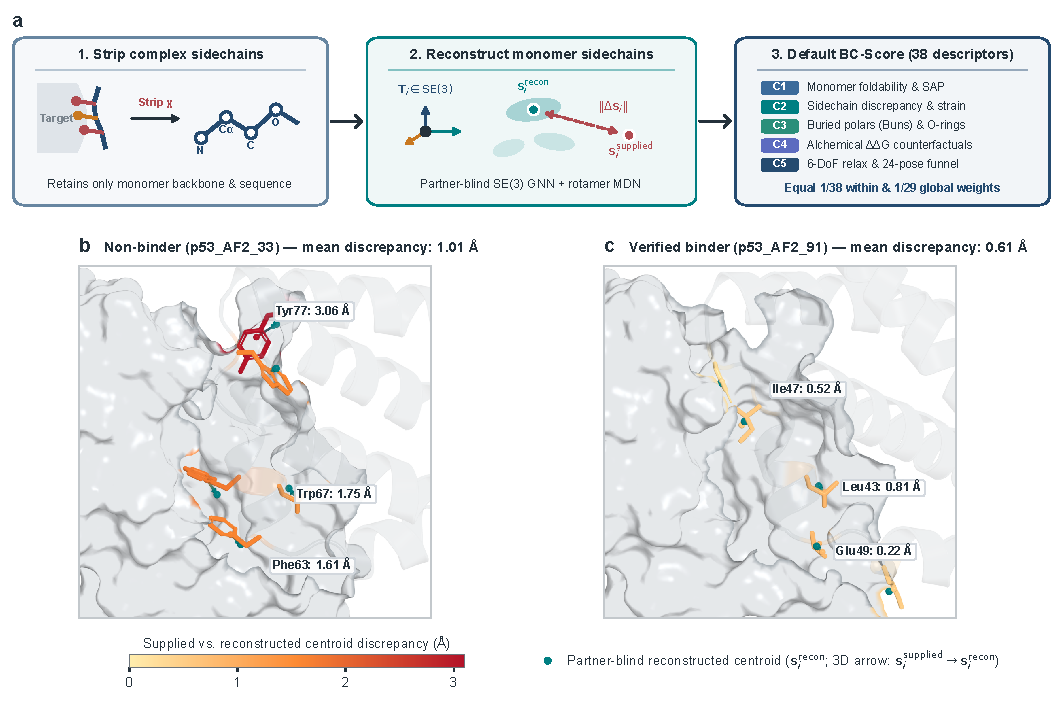
\includegraphics[width=0.92\textwidth]{figures/fig1_pipeline_and_mdm2.pdf}
    \caption{\textbf{BC-Score pipeline and model-predicted sidechain reconstruction discrepancy at designed Mdm2 interfaces.}
    \textbf{a}, Three-stage \texttt{BC-Score} evaluation: (1) supplied sidechains are stripped from the input complex PDB structure, retaining only monomer backbone atoms ($\text{N}, \text{C}_\alpha, \text{C}, \text{O}$) and sequence; (2) a pretrained partner-free $\text{SE}(3)$-equivariant GNN and $K=3$ rotamer Mixture Density Network (MDN) predict monomer-conditioned sidechain centroids $\mathbf{s}_i^{\text{recon}}$, functional tips $\mathbf{t}_i^{\text{recon}}$, and model-derived packing discrepancy $\|\Delta\mathbf{s}_i\| = \|\mathbf{s}_i^{\text{recon}} - \mathbf{s}_i^{\text{supplied}}\|$; and (3) default \texttt{BC-Score} combines $38$ within-target and $29$ cross-target descriptors across five physical modules (C1--C5) using equal $1/38$ within-target and $1/29$ cross-target descriptor weights without benchmark-fitted feature weights ($0.043\,\text{s}$ per complex in batched A100 GPU evaluation; the five-module macro-average variant \texttt{BC-Score-5M} averages the five module sub-scores at $1/5$ each and includes a fourth C4 cross-target inverse-folding term [$30$ cross-target descriptors total]).
    \textbf{b, c}, Interface close-ups of an experimentally tested Mdm2 non-binder (\texttt{p53\_AF2\_33}, \textbf{b}; $n = 1$ complex) and verified binder (\texttt{p53\_AF2\_91}, \textbf{c}; $n = 1$ complex) from the Overath et al.\ benchmark ($n = 3,532$ complexes; two-sided Mann--Whitney $U$ test on interface strain $Z_{\text{strain}}$, $P = 1.1\times 10^{-4}$). Interface residues are colored by centroid reconstruction discrepancy on a shared $0\text{--}3.1\,\text{\AA}$ blue-to-red colour scale ($1.01\,\text{\AA}$ full-interface mean for the non-binder versus $0.61\,\text{\AA}$ for the binder), with 3D displacement arrows connecting complex-packed supplied centroids ($\mathbf{s}_i^{\text{supplied}}$) to partner-blind reconstructed centroids ($\mathbf{s}_i^{\text{recon}}$, filled teal spheres).}
    \label{fig:mirage}
\end{figure*}

Here we introduce the \textbf{Backbone-Conditioned Sidechain Reconstruction Score (\texttt{BC-Score})}, a fast scoring function that strips non-backbone atoms from each chain and applies a three-layer $\text{SE}(3)$-equivariant GNN \cite{satorras2021egnn,jing2021gvp} pretrained on crystal monomers \cite{kringelum2012discotope,dunbar2014sabdab} (Fig.~\ref{fig:mirage}a). From monomer backbone geometry ($\text{N}, \text{C}_\alpha, \text{C}, \text{O}, \text{C}_\beta$) and sequence alone, the network predicts each residue's expected sidechain centroid $\hat{\mathbf{s}}_i^{\text{recon}}$, distal functional tip $\hat{\mathbf{t}}_i^{\text{recon}}$, and a $K=3$ Mixture Density Network (MDN) \cite{bishop1994mdn} over $\chi_1$ rotamer modes $\{\pi_{i,k}, \hat{\mathbf{s}}_{i,k}^{\text{recon}}, \hat{\mathbf{t}}_{i,k}^{\text{recon}}\}_{k=1}^3$ \cite{shapovalov2011dunbrack}. Comparing $\hat{\mathbf{s}}_i^{\text{recon}}$ with $\mathbf{s}_i^{\text{supplied}}$ yields a model-derived proxy for packing inconsistency---the \textbf{sidechain reconstruction discrepancy} $\|\hat{\mathbf{s}}_i^{\text{recon}} - \mathbf{s}_i^{\text{supplied}}\|$ and minimum-mode rotamer distance $\min_k \|\hat{\mathbf{s}}_{i,k}^{\text{recon}} - \mathbf{s}_i^{\text{supplied}}\|$ (Fig.~\ref{fig:mirage}b,c)---while providing partner-blind sidechain coordinates for interface scoring.

Default \texttt{BC-Score} combines $38$ within-target descriptors (weighted equally at $1/38$) and $29$ cross-target descriptors (weighted equally at $1/29$, with zero feature weights fitted on benchmark targets) organized into five physical modules: (C1) monomer foldability, 3D inverse-folding compatibility, and Spatial Aggregation Propensity (\texttt{SAP}) \cite{chennamsetty2009sap}; (C2) sidechain reconstruction discrepancy, rotamer strain proxies, and autograd backbone restoring forces ($\nabla_{\mathbf{X}} \log P_{\text{IF}}(\mathbf{s}\mid\mathcal{G})$); (C3) bilateral buried unsatisfied polar (``Buns'') penalties \cite{coventry2021buried}, burial-screened electrostatics, and aromatic O-ring packing \cite{bogan1998anatomy}; (C4) in-place alchemical sequence counterfactuals, Alanine scanning, and holo-versus-apo inverse-folding log-odds; and (C5) continuous six-degree-of-freedom (6-DoF) rigid-body relaxation and 24-pose $\text{SE}(3)$ re-docking funnel sharpness under a pretrained pairwise interface potential. Unless explicitly labeled otherwise, \texttt{BC-Score} refers to this default descriptor-level equal-weight model ($38$ within-target and $29$ cross-target descriptors); as sensitivity analyses, we also report a five-module macro-average variant that averages the five module sub-scores at $1/5$ each and includes an additional C4 cross-target inverse-folding term ($30$ cross-target descriptors total; \texttt{BC-Score-5M}), inner-Leave-One-Target-Out (LOTO) shrinkage-regularized descriptor weights on the default $38$-within-target and $29$-cross-target descriptor set (\texttt{BC-Score [Reg.\ LOTO]}), and a cohort-free single-complex ($M=1$) thermodynamic-cycle formulation (\texttt{True-EBM}).

\section{Results}

\subsection{Backbone-conditioned sidechain reconstruction}
On $60$ held-out crystal validation monomers ($12,248$ residues) and $50$ crystal complexes, our 2-Point $\text{SE}(3)$ GNN reduces sidechain centroid Mean Absolute Error (MAE) from $0.89\,\text{\AA}$ to $0.48\,\text{\AA}$ ($86.0\%$ versus $65.6\%$ within $1.0\,\text{\AA}$) and distal tip MAE from $1.59\,\text{\AA}$ to $0.86\,\text{\AA}$ relative to a canonical rigid-backbone local-frame template (Extended Data Table~\ref{tab:reconstruction}). The largest gain occurs on bulky aromatics ($\text{Phe}, \text{Trp}, \text{Tyr}$), where centroid MAE drops from $2.13\,\text{\AA}$ to $0.58\,\text{\AA}$ and tip MAE drops from $3.81\,\text{\AA}$ to $0.90\,\text{\AA}$; at crystal complex interfaces ($<8.5\,\text{\AA}$ $\text{C}_\alpha$), centroid MAE is $0.57\,\text{\AA}$ versus $1.05\,\text{\AA}$ for the template.

Across the Overath et al.\ benchmark ($n=3,532$; $391$ binders, $3,141$ non-binders; Fig.~\ref{fig:mirage}b,c), model-predicted discrepancy between supplied and reconstructed sidechains is higher at interface residues than at non-interface surface residues on the same monomer (two-sided paired Wilcoxon signed-rank test, $P = 1.4\times 10^{-13}$). Between outcomes, experimental non-binders exhibit larger within-target interface discrepancy ($P = 1.5\times 10^{-3}$) and a higher uncertainty-normalized strain proxy ($Z_{\text{strain}} = +0.14$ versus $-0.07$, two-sided Mann--Whitney $U$ test, $P = 1.1\times 10^{-4}$) than verified binders. Because $\hat{\mathbf{s}}_i^{\text{recon}}$ is predicted from static crystal monomer backbones rather than experimental unbound structures, we interpret $Z_{\text{strain}}$ as a statistical packing-inconsistency signal rather than a direct physical measurement of unbound conformational strain.

\subsection{Standalone benchmark across 13 targets}
We evaluated standalone \texttt{BC-Score} (operating strictly on input design PDB structures without co-folding) against \texttt{PyRosetta} $\Delta G_{\text{sep}}$ \cite{chaudhury2010pyrosetta,alfort2017rosetta}, \texttt{SpatialPPI v2} \cite{spatialppi2}, and seven co-folding metrics from Overath et al.\ \cite{overath2025predicting} across all $3,532$ complexes and $13$ targets under LOTO cross-validation (Table~\ref{tab:benchmark}, Fig.~\ref{fig:benchmark}, and Extended Data Table~\ref{tab:ext_benchmark}). Co-folding baselines include \texttt{AlphaFold2} initial-guess interface predicted Aligned Error (\texttt{iPAE}) \cite{bennett2023improving}, \texttt{ColabFold AF2-Multimer} \cite{evans2021afmultimer,mirdita2022colabfold} interface predicted Structural Aligned Error (\texttt{ipSAE}) \cite{dunbrack2025ipsae} and active interface predicted Template Modeling score (\texttt{actifpTM}) \cite{varga2025actifptm}, \texttt{Boltz-1 ipSAE} \cite{wohlwend2024boltz1,dunbrack2025ipsae}, and \texttt{AlphaFold3} \cite{abramson2024accurate} interface predicted Template Modeling score (\texttt{ipTM}), Local Interaction Score (\texttt{LIS}) \cite{kim2024lis}, and \texttt{ipSAE}.

\begin{figure*}[!t]
    \centering
    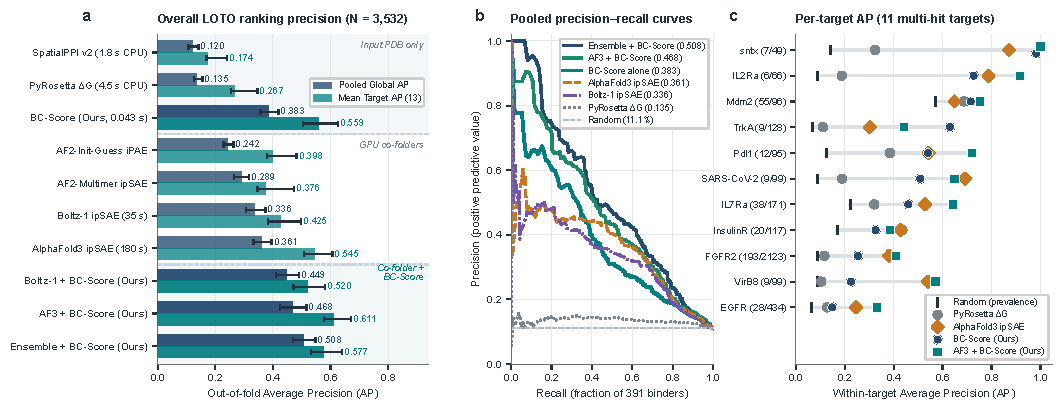
\includegraphics[width=\textwidth]{figures/fig2_loto_benchmark.pdf}
    \caption{\textbf{Leave-One-Target-Out (LOTO) ranking performance across 3,532 experimentally tested de novo binders.}
    \textbf{a}, Out-of-fold Pooled Global AP (filled navy bars, point estimate) and unweighted 13-target Mean Target AP (filled teal bars, mean across $13$ targets) with error bars indicating $95\%$ target-stratified paired bootstrap confidence intervals ($B = 10,000$ resamples across $n = 3,532$ complexes; two-sided paired bootstrap $P < 0.001$ for standalone \texttt{BC-Score} versus \texttt{PyRosetta} $\Delta G_{\text{sep}}$, \texttt{SpatialPPI v2}, \texttt{AF2-Init-Guess iPAE}, and \texttt{AF2-Multimer ipSAE}; $P = 0.036$ versus \texttt{Boltz-1 ipSAE}; $P = 0.338$ versus \texttt{AlphaFold3 ipSAE}; Table~\ref{tab:benchmark} and Extended Data Table~\ref{tab:ext_benchmark}). The vertical grey dashed line marks random baseline prevalence ($0.111$).
    \textbf{b}, Pooled out-of-fold precision--recall curves across all $n = 3,532$ candidates ($391$ verified binders; horizontal grey dashed line indicates random prevalence $11.1\%$).
    \textbf{c}, Within-target out-of-fold AP across the $11$ multi-hit receptor campaigns ($\ge 6$ binders per target, $n = 3,477$ of $3,532$ designs), with positive counts $(n_{\text{pos}}/N_t)$ indicated in each y-axis label and target-specific random prevalence marked by vertical black tick marks.}
    \label{fig:benchmark}
\end{figure*}

Across all $3,532$ complexes, standalone \texttt{BC-Score} nearly triples the Pooled Global AP of \texttt{PyRosetta} $\Delta G_{\text{sep}}$ and \texttt{SpatialPPI v2} ($0.383$ versus $0.135$ and $0.120$, $\Delta = +0.248$, $P < 0.001$, Benjamini--Hochberg false discovery rate [FDR] $q = 0.001$; 13-target Mean $\text{AP} = 0.559$ versus $0.267$ and $0.174$; Table~\ref{tab:benchmark} and Fig.~\ref{fig:benchmark}a). Across formulation and weighting variants, shrinkage-regularized inner-LOTO descriptor weights on the identical $38$-within-target and $29$-cross-target descriptor set yield $\text{Pooled AP} = 0.382$ ($\Delta = -0.001$ versus default equal descriptor weights, $P = 0.786$; $0.560$ Mean Target AP), while the five-module macro-average variant (\texttt{BC-Score-5M}, which both weights the five module sub-scores at $1/5$ each and includes a fourth C4 cross-target term) reaches $\text{Pooled AP} = 0.366$ ($0.527$ Mean Target AP; Extended Data Table~\ref{tab:ext_benchmark}).

Compared against GPU co-folders, standalone \texttt{BC-Score} exceeds \texttt{AlphaFold2-Initial-Guess iPAE}, \texttt{ColabFold AF2-Multimer ipSAE} and \texttt{actifpTM}, \texttt{AlphaFold3 ipTM}, and \texttt{Boltz-1 ipSAE} on Pooled Global AP ($0.383$ versus $0.242\text{--}0.336$, all $P \le 0.036$, BH $q \le 0.046$) and 13-target Mean AP ($0.559$ versus $0.376\text{--}0.480$). Against \texttt{AlphaFold3 LIS} ($0.350$, $P = 0.126$) and \texttt{AlphaFold3 ipSAE} ($\text{Pooled AP} = 0.361$, $\Delta = +0.022$, $95\%$ confidence interval [CI] $[-0.023, +0.064]$, $P = 0.338$; 13-target Mean $\text{AP} = 0.545$, $\Delta = +0.014$, $P = 0.802$), the observed differences are not statistically significant across the $13$ targets, which indicates comparable precision on this cohort without establishing formal statistical equivalence. Excluding \texttt{FGFR2} ($2,123$ of $3,532$ designs) widens the pooled difference between \texttt{BC-Score} and both \texttt{Boltz-1 ipSAE} and \texttt{AlphaFold3 ipSAE} ($0.487$ versus $0.353$ and $0.390$). Across the $11$ multi-hit campaigns ($\ge 6$ binders), \texttt{BC-Score} achieves a Mean AP of $0.502$ versus $0.430$ for \texttt{Boltz-1 ipSAE}, $0.496$ for \texttt{AlphaFold3 LIS}, and $0.543$ for \texttt{AlphaFold3 ipSAE} (Fig.~\ref{fig:benchmark}b,c).

Performance holds on receptors non-homologous to the pretraining corpus (Smith--Waterman local identity $<30\%$; Section~\ref{sec:pretraining}): across the $10$ targets with $<30\%$ identity to the interface training set ($n=2,933$), \texttt{BC-Score} achieves $\text{Pooled AP} = 0.401$ and $\text{Mean Target AP} = 0.590$ (versus $0.367$ and $0.536$ for \texttt{AlphaFold3 ipSAE}), and across the $5$ targets with $<30\%$ identity to both monomer and interface corpora ($n=2,326$), Mean Target AP is $0.643$ (versus $0.582$ for \texttt{AlphaFold3 ipSAE} and $0.206$ for \texttt{PyRosetta} $\Delta G_{\text{sep}}$).

\subsection{Sidechain attribution and component dissection}
To isolate the contribution of reconstructed sidechains across all $3,532$ complexes (Fig.~\ref{fig:heatmap}a), we compared a monomer-backbone-only baseline (\texttt{C1} alone; $\text{Pooled AP} = 0.199$, 11-target $\text{Mean AP} = 0.226$) against three matched five-module (\texttt{C1}--\texttt{C5}) evaluations that hold standardization, the 24-pose $\text{SE}(3)$ re-docking grid, and the five alchemical counterfactuals fixed while varying only the sidechain coordinate source: canonical rigid-template sidechains $\hat{\mathbf{s}}_i^{\text{template}}$ ($0.265$, $0.344$), complex-packed supplied sidechains $\mathbf{s}_i^{\text{supplied}}$ ($0.281$, $0.381$), and partner-blind GNN-reconstructed sidechains $\hat{\mathbf{s}}_i^{\text{recon}}$ in \texttt{BC-Score} ($0.383$, $0.502$), which improves Pooled Global AP by $+0.102$ and 11-target Mean AP by $+0.121$ over supplied sidechains (both $P < 0.001$).

\begin{figure*}[!t]
    \centering
    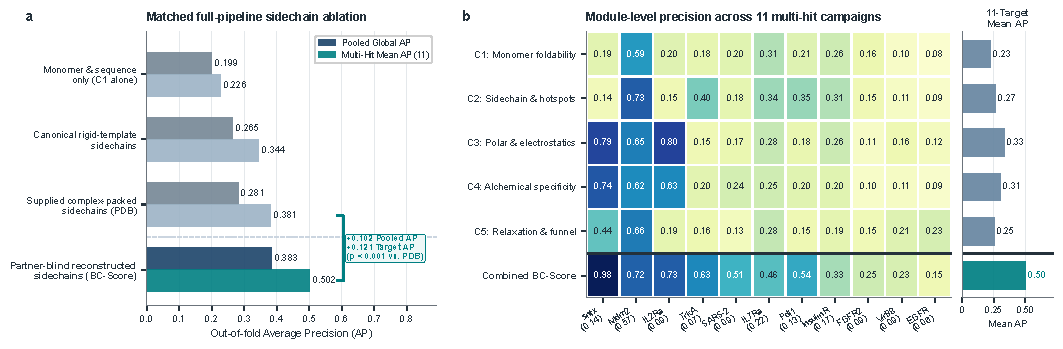
\includegraphics[width=\textwidth]{figures/fig3_sidechain_ablation_and_modules.pdf}
    \caption{\textbf{Sidechain attribution ablation and module-level precision across 11 multi-hit campaigns.}
    \textbf{a}, Out-of-fold Pooled Global AP (filled navy bars, left) and 11-target Multi-Hit Mean AP (filled teal bars, right) with error bars showing $95\%$ target-stratified paired bootstrap confidence intervals ($B = 10,000$ resamples across $n = 3,532$ complexes; two-sided paired bootstrap $P < 0.001$ for partner-blind GNN-reconstructed sidechains $\hat{\mathbf{s}}_i^{\text{recon}}$ versus supplied sidechains $\mathbf{s}_i^{\text{supplied}}$, rigid-backbone template $\hat{\mathbf{s}}_i^{\text{template}}$, and monomer-only \texttt{C1}).
    \textbf{b}, Heat map of within-target AP for each physical module (C1--C5) and combined \texttt{BC-Score} across the $11$ multi-hit campaigns ($n = 3,477$ complexes; positive prevalence in parentheses), with right-hand horizontal bars showing the unweighted 11-target Mean AP.}
    \label{fig:heatmap}
\end{figure*}

Across the $11$ multi-hit campaigns, different modules lead on different targets relative to positive prevalence ($0.065\text{--}0.573$; Fig.~\ref{fig:heatmap}b): sidechain discrepancy and rotamer strain (C2) lead on five targets (\texttt{Mdm2}, \texttt{TrkA}, \texttt{Pdl1}, \texttt{IL7Ra}, \texttt{InsulinR}), polar satisfaction (C3) leads on polar interfaces (\texttt{IL2Ra}, \texttt{sntx}), monomer foldability (C1) leads on \texttt{FGFR2}, alchemical specificity (C4) leads on \texttt{SARS-CoV-2 RBD}, and pose funnel sharpness (C5) leads on \texttt{EGFR} and \texttt{VirB8}.

\subsection{Two-stage screening cascades and hybrid reranking}
We evaluated \texttt{BC-Score} as a Stage-1 pre-filter before GPU co-folding and as a Stage-2 hybrid score across retention budgets $\rho \in [0\%, 100\%]$ (Fig.~\ref{fig:hybrids}, Extended Data Fig.~\ref{fig:focused_support}a--c, and Extended Data Table~\ref{tab:cascade}).

\begin{figure*}[!t]
    \centering
    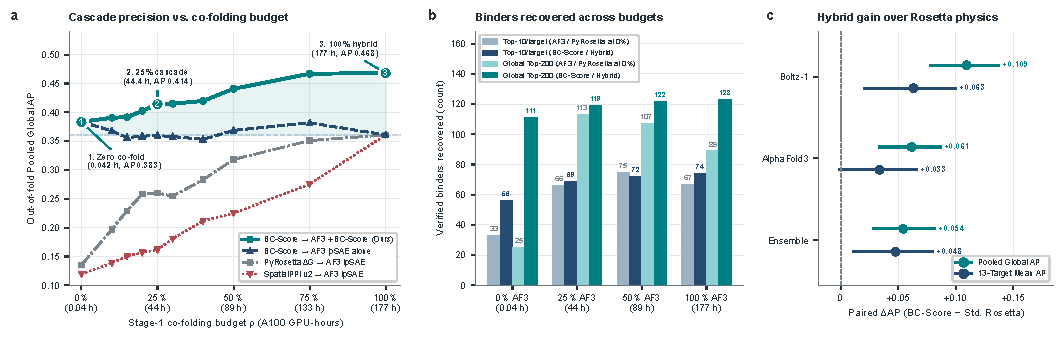
\includegraphics[width=\textwidth]{figures/fig4_cascade_and_hybrids.pdf}
    \caption{\textbf{Two-stage screening cascades and post-co-fold hybrid reranking across 3,532 candidates.}
    \textbf{a}, Out-of-fold Pooled Global AP across Stage-1 co-folding retention budgets $\rho \in [0\%, 100\%]$ ($0.042\text{--}176.6$ A100 GPU-hours across $n = 3,532$ complexes), comparing \texttt{BC-Score} (solid teal and navy curves), \texttt{PyRosetta} $\Delta G_{\text{sep}}$ (orange dashed curve), and \texttt{SpatialPPI v2} (red dotted curve) pre-filters followed by \texttt{AlphaFold3 ipSAE} alone or the \texttt{AlphaFold3 + BC-Score} hybrid (numbered circles denote Operating Points \textbf{1}: $0\%$ co-folding; \textbf{2}: $25\%$ cascade; \textbf{3}: $100\%$ hybrid).
    \textbf{b}, Verified binders recovered in the Top-10 per target ($13$ targets, maximum $130$) and Global Top-200 ($n = 3,532$) at $\rho \in \{0\%, 25\%, 50\%, 100\%\}$ (colored bars indicate method and budget).
    \textbf{c}, Point estimates (filled circles) and horizontal error bars showing $95\%$ target-stratified paired bootstrap confidence intervals ($B = 10,000$ resamples across $n = 3,532$ complexes) for Paired $\Delta\text{AP}$ (Pooled Global AP in teal, 13-Target Mean AP in navy; all two-sided paired bootstrap $P < 0.001$) when augmenting \texttt{Boltz-1}, \texttt{AlphaFold3}, or their ensemble with \texttt{BC-Score} instead of standard Rosetta physical descriptors (vertical grey dashed line marks $\Delta\text{AP} = 0$).}
    \label{fig:hybrids}
\end{figure*}

At \textbf{Operating Point 1 ($\rho = 0\%$, $0.042$ A100 GPU-hours)}, standalone \texttt{BC-Score} without co-folding recovers $56$ top-10-per-target and $111$ global top-200 binders, exceeding unfiltered \texttt{AlphaFold3 ipSAE} on global top-200 recovery ($89$ hits) as well as \texttt{PyRosetta} $\Delta G_{\text{sep}}$ ($25$) and \texttt{SpatialPPI v2} ($32$; Fig.~\ref{fig:hybrids}b and Extended Data Table~\ref{tab:cascade}).

At \textbf{Operating Point 2 ($\rho = 25\%$, $44.4$ A100 GPU-hours)}, Stage-1 \texttt{BC-Score} retains $52.2\%$ of all $391$ binders globally ($47.8\%$ discarded; $64.3\%$ mean across targets) versus $35.8\%$ for \texttt{PyRosetta} $\Delta G_{\text{sep}}$ and $21.2\%$ for \texttt{SpatialPPI v2} (Extended Data Fig.~\ref{fig:focused_support}c). Despite this $52.2\%$ overall recall cutoff, ranking the $25\%$ survivors with \texttt{AlphaFold3 ipSAE} alone yields $66$ top-10-per-target hits (versus $67$ from unfiltered \texttt{AlphaFold3}: $45$ of the original $67$ top-10 hits survive Stage~1 while $22$ are filtered out, and $21$ other surviving true binders move into the top~10 after high-\texttt{ipSAE} non-binders are removed) and $113$ global top-200 hits ($69$ and $119$ with the \texttt{AlphaFold3 + BC-Score} hybrid, $\text{Pooled AP} = 0.414$). At $\rho = 50\%$ ($88.5$ GPU-hours, $76.7\%$ recall), \texttt{AlphaFold3 ipSAE} alone recovers more top-10-per-target hits than the hybrid ($75$ versus $72$), whereas the hybrid recovers more global top-200 hits ($122$ versus $107$; Extended Data Table~\ref{tab:cascade}).

At \textbf{Operating Point 3 ($\rho = 100\%$, $176.6$ A100 GPU-hours)}, combining \texttt{BC-Score} with co-folder confidence under LOTO cross-validation raises Pooled Global AP to $0.449$ with \texttt{Boltz-1}, $0.468$ with \texttt{AlphaFold3} (13-target Mean $\text{AP} = 0.611$), and $0.508$ with their ensemble (all $P < 0.001$; Table~\ref{tab:benchmark}), outperforming standard Rosetta descriptors (\texttt{SAP} \cite{chennamsetty2009sap}, \texttt{CamSol} \cite{sormanni2015camsol}, $\Delta G_{\text{sep}}$, and $\Delta G_{\text{sep}}$ per buried Solvent-Accessible Surface Area [$\Delta G_{\text{sep}}/\Delta\text{SASA}$]; $\Delta\text{AP} = +0.054\text{--}0.109$; Fig.~\ref{fig:hybrids}c and Extended Data Fig.~\ref{fig:focused_support}a,b).

\subsection{Same-epitope discrimination and in silico partition-function co-design}
Across same-target binder and non-binder pairs sharing $\ge 50\%$ ($326,474$ pairs) to $\ge 90\%$ ($4,124$ pairs) Jaccard contact overlap ($\text{C}_\alpha < 8.5\,\text{\AA}$), \texttt{BC-Score} ranks the verified binder higher in $67.2\%\text{--}73.9\%$ of pairs ($66.5\%\text{--}72.7\%$ for \texttt{BC-Score-5M}), beating \texttt{PyRosetta} $\Delta G_{\text{sep}}$ ($59.9\%\text{--}64.3\%$), supplied-sidechain scoring ($58.0\%\text{--}60.0\%$), \texttt{ESM-2} \cite{lin2023evolutionary} ($54.9\%\text{--}56.6\%$), and backbone inverse folding ($49.9\%\text{--}52.1\%$; Extended Data Fig.~\ref{fig:codesign}).

To test whether the potential can guide computational sequence redesign on fixed backbones ($39$ failed Overath scaffolds, $3$ per target; Extended Data Figs.~\ref{fig:focused_support}d--f and~\ref{fig:pose_diagnostic}), we compared single-pose energy minimization $E(\mathbf{x}_0, \mathbf{s})$ ($\sim 0.12\,\text{s}$ per complex) against partition-function free-energy minimization. Optimizing $E(\mathbf{x}_0, \mathbf{s})$ alone improves the single-pose score on $35$ of $39$ scaffolds (two-sided Wilcoxon signed-rank test, $P = 1.3\times 10^{-9}$) and Buns on $31$ of $39$ ($P = 3.7\times 10^{-6}$), but degrades 24-pose funnel Root-Mean-Square Deviation (RMSD) on $19$ of $39$ scaffolds ($20$ of $39$ improved, $P = 0.72$) via apolar mutations that also stabilize decoy poses (Extended Data Fig.~\ref{fig:pose_diagnostic}a). Minimizing the partition-function free energy $\Delta F_{\text{pose}}(\mathbf{x}_0, \mathbf{s}) = E_\theta(\mathbf{x}_0, \mathbf{s}) + \tau \log\!\big(\frac{1}{M_{\text{dec}}}\sum_{m \in \text{Decoy}} e^{-E_\theta(\mathbf{x}_m, \mathbf{s})/\tau}\big)$ over the 24-pose $\text{SE}(3)$ ensemble resolves this in silico mode: it lowers interface energy on $34$ of $39$ scaffolds ($P = 2.1\times 10^{-8}$), reduces Buns on $33$ of $39$ ($P = 8.9\times 10^{-8}$), increases Alanine-scan $\Delta\Delta G$ on $34$ of $39$ ($+1.01 \to +2.10$, $P = 2.1\times 10^{-8}$), improves frozen monomer inverse-folding log-likelihood on $38$ of $39$ ($P = 7.3\times 10^{-12}$), sharpens the 24-pose funnel on $\mathbf{37}$ of $\mathbf{39}$ scaffolds ($0.95\,\text{\AA} \to 0.74\,\text{\AA}$, $P = 2.3\times 10^{-9}$; Extended Data Fig.~\ref{fig:pose_diagnostic}b), and reduces pose-funnel RMSD by $52.4\%$ ($2.22\,\text{\AA} \to 1.06\,\text{\AA}$) on an independent held-out 24-pose $\text{SE}(3)$ verification ensemble across $\mathbf{33}$ of $\mathbf{39}$ scaffolds ($P = 1.3\times 10^{-4}$). These results demonstrate computational objective consistency across held-out poses, not experimental wet-lab rescue.

\subsection{Held-out external validation}
Using the frozen Overath checkpoints and normalization parameters (Section~\ref{sec:reproducibility}), we evaluated two held-out public campaigns (Fig.~\ref{fig:external} and Extended Data Table~\ref{tab:external}): (1) \textbf{\texttt{Nipah-G}}, from the Adaptyv Bio and Proteinbase \textit{Nipah Competition Results} collection (\texttt{nipah-binder-competition-results}, \url{https://proteinbase.com/collections/nipah-binder-competition-results}; $n=881$ expressed candidates with \texttt{Boltz-2} complex predictions \cite{passaro2025boltz2} after excluding $146$ non-expressed, $2$ structure-missing, and $1$ conflicting entry from the $1,030$ evaluated submissions, yielding $100$ surface plasmon resonance [SPR] binders [$11.35\%$]); and (2) \textbf{\texttt{Scorpion}}, from the Anthropic and Adaptyv Bio scorpion toxin binder design dataset (\texttt{Anthropic/scorpion-toxin-binder-design}, \url{https://huggingface.co/datasets/Anthropic/scorpion-toxin-binder-design}; $n=243$ raw pre-co-fold design PDB structures across $5$ neurotoxins [receptor target structures from PDB \texttt{25IH}, \texttt{1NPI}, \texttt{1AHO}, \texttt{7K18} and AlphaFold Database \texttt{AF-P01479-F1}] generated using \texttt{Mosaic}, \texttt{PXDesign}, \texttt{Genie 3}, \texttt{RFdiffusion3} and \texttt{RFdiffusion} \cite{watson2023de}, \texttt{Proteina-Complexa}, \texttt{FreeBindCraft} \cite{pacesa2024bindcraft}, \texttt{BoltzGen} \cite{stark2025boltzgen}, \texttt{Protein Hunter}, and \texttt{BoltzDesign1}; $21$ Adaptyv SPR hits [$8.64\%$] and $12$ Twist-confirmed publication hits [$4.94\%$]).

\begin{figure*}[!t]
    \centering
    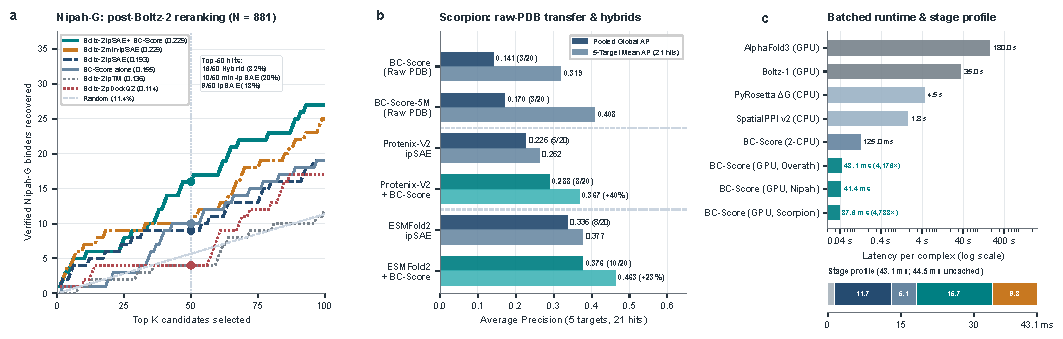
\includegraphics[width=\textwidth]{figures/fig5_external_and_runtime.pdf}
    \caption{\textbf{Held-out external validation across two public campaigns and batched runtime profiling.}
    \textbf{a}, Cumulative verified binders recovered in the top $K \in [1, 100]$ selections on the Adaptyv Bio \texttt{Nipah-G} campaign ($n = 881$ \texttt{Boltz-2} complexes, $100$ binders; grey dotted line marks random expectation), comparing standalone default \texttt{BC-Score} (solid blue curve), \texttt{Boltz-2} confidence metrics (navy dashed, orange dash-dotted, grey dotted, and red dotted curves), and the locked \texttt{Boltz-2 ipSAE + BC-Score} hybrid (solid teal curve; $95\%$ bootstrap confidence intervals [$B = 10,000$ resamples] for Pooled AP are reported in Extended Data Table~\ref{tab:external}).
    \textbf{b}, Point estimates for Pooled Global AP (dark navy and dark teal bars, with Top-20 hit counts in parentheses) and unweighted 5-target Mean Target AP (light blue and light teal bars) across $n = 243$ raw pre-co-fold \texttt{Scorpion} neurotoxin design PDB structures ($5$ targets, $21$ Adaptyv hits; sensitivity metrics on the $12$ Twist-confirmed publication hits are reported in brackets in Extended Data Table~\ref{tab:external}).
    \textbf{c}, Mean batched per-complex latency (log scale, horizontal bars) across GPU co-folders ($n = 3,532$), CPU baselines ($n = 100$), and \texttt{BC-Score} ($n = 100$ complexes on Overath, $n = 881$ on \texttt{Nipah-G}, $n = 243$ on \texttt{Scorpion}), with the A100 GPU stage profile below ($41.75\,\text{ms}$ across five GPU compute passes plus $1.35\,\text{ms}$ cached-target coordinate setup and transfer $= 43.10\,\text{ms}$ batched wall-clock; replacing cached setup with full uncached raw-PDB parsing of both chains [$2.70\,\text{ms}$] gives $41.75 + 2.70 = 44.45\,\text{ms}$).}
    \label{fig:external}
\end{figure*}

External performance is metric- and variant-dependent (Extended Data Table~\ref{tab:external}). On \textbf{\texttt{Nipah-G}} ($0.041\,\text{s}$ per complex in batched A100 evaluation), standalone default \texttt{BC-Score} achieves $\text{AP} = 0.155$ and $10/50$ top-50 hits ($0.156$ and $11/50$ with regularized LOTO weights; $M=1$ \texttt{True-EBM} reaches $\text{AP} = 0.182$, $11/50$ top-50 hits), outperforming \texttt{ProteinMPNN} \cite{dauparas2022robust}, \texttt{ESMFold} monomer predicted Local Distance Difference Test (pLDDT) \cite{lin2023evolutionary}, and \texttt{Boltz-2} \texttt{pDockQ2} \cite{bryant2022pdockq,zhu2023pdockq2}, \texttt{LIS} \cite{kim2024lis}, \texttt{ipTM}, and complex pLDDT ($\text{AP} = 0.100\text{--}0.146$), while trailing standalone \texttt{Boltz-2 ipSAE} ($\text{AP} = 0.193$, Area Under the Receiver Operating Characteristic curve [$\text{AUROC}$] $= 0.622$, $7/25$ top-25, $9/50$ top-50) and $\min\text{ipSAE}$ ($\text{AP} = 0.229$, $\text{AUROC} = 0.645$, $9/25$ top-25, $10/50$ top-50; Fig.~\ref{fig:external}a). Combining default \texttt{BC-Score} with \texttt{Boltz-2 ipSAE} raises AP by $+18.7\%$ ($0.193 \to 0.229$) and top-50 hits from $9/50$ ($18\%$) to $\mathbf{16/50}$ ($32.0\%$), tying $\min\text{ipSAE}$ in AP while trailing $\min\text{ipSAE}$ in AUROC ($0.618$ versus $0.645$) and top-25 hits ($8/25$ versus $9/25$).

On \textbf{\texttt{Scorpion}} ($n=243$ raw pre-co-fold PDB structures across $5$ targets), standalone default \texttt{BC-Score} ($\text{Pooled AP} = 0.141$, $\text{AUROC} = 0.618$, $3/20$ top-20, $7/50$ top-50) and \texttt{BC-Score-5M} ($\text{Pooled AP} = 0.170$, $\text{AUROC} = 0.609$, $3/20$ top-20, $7/50$ top-50) trail standalone co-folders (\texttt{Protenix-V2 ipSAE} \cite{bytedance2025protenix} $\text{Pooled AP} = 0.226$, $5/20$ top-20, $11/50$ top-50; \texttt{ESMFold2 ipSAE} \cite{candido2026esmfold2} $\text{Pooled AP} = 0.336$, $8/20$ top-20, $16/50$ top-50; self-consistency \texttt{DockQ} [\texttt{scDockQ}] \cite{basu2016dockq} baselines are shown in Extended Data Table~\ref{tab:external}). One possible explanation for this lower pooled standalone precision is that the supplied \texttt{Scorpion} coordinates combine unrelaxed pre-co-fold structures across ten upstream generators in small per-target cohorts ($N_t = 38\text{--}66$), which may shift cross-target descriptor baselines relative to uniformly relaxed Overath complexes, although differences in target difficulty, small-toxin receptor geometry, and assay definitions may also contribute. Within targets, default \texttt{BC-Score} reaches $0.319$ 5-target Mean AP ($0.448$ on the $12$ publication hits) and \texttt{BC-Score-5M} reaches $0.408$ ($0.599$ on publication hits, driven by ranking both \texttt{LqhIII} hits at positions 1--2; across the four targets with $\ge 3$ hits, \texttt{BC-Score} and \texttt{BC-Score-5M} achieve $0.316$ and $0.261$ versus $0.281$ for \texttt{Protenix-V2} and $0.347$ for \texttt{ESMFold2}; Fig.~\ref{fig:external}b). Post-co-fold hybrids improve early precision and within-target AP for both co-folders---\texttt{Protenix-V2 + BC-Score} lifts Pooled AP ($0.226 \to 0.288$), 5-target Mean AP ($0.262 \to 0.367$; $0.224 \to 0.415$ on publication hits), and top-20 hits ($5/20 \to 8/20$), while \texttt{ESMFold2 + BC-Score} lifts Pooled AP ($0.336 \to 0.376$), 5-target Mean AP ($0.377 \to 0.463$; $0.386 \to 0.527$ on publication hits), and top-20 hits ($8/20 \to 10/20$)---but exhibit lower global AUROC ($0.706$ versus $0.748$ and $0.785$ versus $0.823$) and equal or lower top-50 recovery ($11/50$ versus $11/50$ for \texttt{Protenix-V2}, and $13/50$ versus $16/50$ for \texttt{ESMFold2}).

\section{Discussion}
Reconstructing monomer-conditioned sidechain geometry from backbone coordinates provides an inexpensive post-design structural signal ($0.038\text{--}0.043\,\text{s}$ per complex in batched A100 GPU evaluation, $4,176\text{--}4,783\times$ faster than \texttt{AlphaFold3} at the post-design scoring step, excluding upstream backbone and sequence generation) that complements all-atom co-folding networks. At the same time, three limitations bound its scope and guide practical deployment: (1) \textbf{Recall versus compute in Stage-1 pre-filtering:} while a $\rho = 25\%$ Stage-1 cutoff recovers $66$ versus $67$ \texttt{AlphaFold3} top-10-per-target hits ($45$ shared plus $21$ newly promoted after filtering out high-\texttt{ipSAE} non-binders), it discards $47.8\%$ of all binders globally ($52.2\%$ recall); campaigns prioritizing overall recall should use $\rho = 50\%$ ($76.7\%$ recall; Extended Data Table~\ref{tab:cascade}) or post-co-fold hybrid reranking ($\rho = 100\%$). (2) \textbf{Reduced standalone transfer on heterogeneous external cohorts:} on \texttt{Scorpion}, pooled standalone \texttt{BC-Score} trails co-folding baselines, potentially reflecting baseline shifts across unrelaxed coordinates from multiple upstream generators, smaller per-target sample sizes, or target-specific effects; in such settings, \texttt{BC-Score} is more effective as a post-co-fold hybrid modifier or via \texttt{BC-Score-5M} for within-target ranking. (3) \textbf{Model-derived proxy and lack of prospective wet-lab validation:} because our GNN is trained on static crystal monomers rather than solution ensembles, sidechain discrepancy is a statistical proxy rather than a direct physical measurement of unbound strain, and all co-design trajectories represent \textit{in silico} objective optimization pending prospective experimental synthesis.

\section{Methods}

\subsection{Pretraining corpus and sequence-identity audit}
\label{sec:pretraining}
All three neural networks within \texttt{BC-Score}---the 3D backbone inverse-folding GNN, the 2-Point sidechain reconstruction GNN, and the pairwise interface potential---were pretrained on crystal structures prior to evaluation on de novo design benchmarks. Combining $900$ crystal structures ($50\text{--}450$ residues) from \texttt{DiscoTope} \cite{kringelum2012discotope} with non-redundant crystal chains from \texttt{SAbDab} \cite{dunbar2014sabdab} clustered via \texttt{MMseqs2} \cite{steinegger2017mmseqs2} ($240$ clusters) yielded $1,288$ monomer chains, split deterministically (seed $2026$) into $1,228$ training and $60$ validation monomers. To form $520$ native-packed training interfaces without de novo designed binders, we combined $360$ cleaved contiguous crystal subdomain interfaces ($40\text{--}58$ residues packing against the remaining core with $\ge 18$ $\text{C}_\alpha$ contacts within $8.5\,\text{\AA}$ and a $\ge 6$-residue cleavage buffer) with $160$ non-redundant \texttt{SAbDab} interfaces.

We quantified sequence overlap with the Overath et al.\ benchmark ($3,532$ complexes, $13$ targets) via Smith--Waterman local alignment ($\text{match} = +1$, $\text{mismatch} = -1$, $\text{gap open} = -2$, $\text{gap extend} = -0.5$, normalized by shorter sequence length). De novo binder sequences have a median maximum local identity of $14.1\%$ to any pretraining chain (Interquartile Range [IQR] $12.8\%\text{--}15.8\%$, 95th percentile $19.4\%$, maximum $30.0\%$). Among the $13$ target receptors, $10$ targets (\texttt{FGFR2}, \texttt{IL10Ra}, \texttt{IL7Ra}, \texttt{InsulinR}, \texttt{LTK}, \texttt{Mdm2}, \texttt{Pdl1}, \texttt{TrkA}, \texttt{VirB8}, \texttt{sntx}; $2,933$ of $3,532$ complexes [$83.0\%$]) share $<30\%$ local identity ($11.5\%\text{--}23.8\%$) with the interface training corpus, while $3$ targets (\texttt{EGFR}, \texttt{IL2Ra}, \texttt{SARS-CoV-2 RBD}) have crystal homologues in \texttt{SAbDab} and \texttt{DiscoTope}. Against the combined monomer and interface corpora, $5$ targets (\texttt{FGFR2} [$15.9\%$], \texttt{IL10Ra} [$17.3\%$], \texttt{LTK} [$19.2\%$], \texttt{VirB8} [$11.5\%$], \texttt{sntx} [$18.3\%$]; $n=2,326$ [$65.9\%$]) have $<30\%$ local identity to every pretraining chain.

\subsection{Network architectures and training hyperparameters}
For each residue $i$, we construct a local frame $\mathbf{T}_i = (\mathbf{R}_i, \mathbf{x}_{i,\text{C}_\alpha}) \in \text{SE}(3)$ from $(\text{N}, \text{C}_\alpha, \text{C})$ via Gram--Schmidt orthogonalization and connect $k=16$ spatial nearest neighbors with $41$ $\text{SE}(3)$-invariant edge features and $57$ node features \cite{satorras2021egnn,jing2021gvp}. All networks were trained in PyTorch using \texttt{AdamW} (weight decay $10^{-4}$, gradient clipping at $1.0$, cosine schedule to $\eta_{\min} = 10^{-4}$, seed $2026$):
\begin{enumerate}
    \item \textbf{3D Backbone Inverse-Folding GNN:} $3$ layers, hidden dimension $96$, dropout $0.10$, trained on backbone coordinates ($\text{N}, \text{C}_\alpha, \text{C}, \text{O}$, ideal $\text{C}_\beta$) for $15$ epochs (batch size $8$, initial learning rate $1.5\times 10^{-3}$, cross-entropy loss with label smoothing $0.05$).
    \item \textbf{2-Point Sidechain Reconstruction GNN:} $3$ layers, hidden dimension $96$, conditioned on backbone geometry and one-hot residue identity $s_i$. It predicts local-frame centroid and tip offsets and uncertainties $(\hat{\mathbf{u}}_i^{\text{cm}}, \hat{\sigma}_i^{\text{cm}}, \hat{\mathbf{u}}_i^{\text{tip}}, \hat{\sigma}_i^{\text{tip}})$ plus a $K=3$ rotamer MDN head $\{\pi_{i,k}, \hat{\mathbf{u}}_{i,k}^{\text{cm}}, \hat{\sigma}_{i,k}^{\text{cm}}, \hat{\mathbf{u}}_{i,k}^{\text{tip}}, \hat{\sigma}_{i,k}^{\text{tip}}\}_{k=1}^3$ \cite{bishop1994mdn,shapovalov2011dunbrack}, trained for $15$ epochs (batch size $8$, learning rate $2.5\times 10^{-3}$) on $\mathcal{L}_{\text{SC}} = \mathcal{L}_{\text{cm-NLL}} + \|\hat{\mathbf{u}}_i^{\text{cm}} - \mathbf{u}_i^{\text{cm}}\|_2^2 + 0.35(\mathcal{L}_{\text{MDN-NLL}} + \mathcal{L}_{\text{MDN-WTA}}) + 0.85(\mathcal{L}_{\text{tip-NLL}} + \|\hat{\mathbf{u}}_i^{\text{tip}} - \mathbf{u}_i^{\text{tip}}\|_2^2 + 0.35[1 - \cos\angle(\hat{\mathbf{u}}_i^{\text{tip}}, \mathbf{u}_i^{\text{tip}})])$.
    \item \textbf{Pairwise Interface Potential:} $2$ monomer GNN layers (hidden dimension $64$) and a 3-layer pairwise multilayer perceptron ($173 \to 64 \to 32 \to 2$) over cross-interface pairs within $10.5\,\text{\AA}$ $\text{C}_\alpha$, using variance-convolved steric widths $\sigma_{\text{eff},ij}^2 = \sigma_0^2 + (\hat{\sigma}_i^{\text{cm}})^2 + (\hat{\sigma}_j^{\text{cm}})^2$ and burial-screened dielectric $\varepsilon(B_{ij})$. Trained for $12$ epochs ($1$ interface with $24$ rigid-body poses and $5$ sequence decoys per batch, learning rate $2.0\times 10^{-3}$) using InfoNCE ($\tau = 0.50$) plus hinge margins $0.5\max(0, E_0 - E_{\text{pose}}^{\min} + 0.50) + 0.6\max(0, E_0 - E_{\text{seq}}^{\min} + 0.35)$ for decoys with $\text{RMSD} > 2.0\,\text{\AA}$.
\end{enumerate}

\subsection{Physical scoring architecture and calibration sensitivity}
Default \texttt{BC-Score} organizes $38$ within-target descriptors $\mathbf{z}_i^{\text{within}} \in \mathbb{R}^{38}$ ($9+9+10+6+4$) and $29$ cross-target descriptors $\mathbf{z}_i^{\text{global}} \in \mathbb{R}^{29}$ ($5+10+5+3+6$) into five modules:
\begin{enumerate}
    \item \textbf{C1 (Monomer foldability; $9$ within-target, $5$ cross-target):} Intra-monomer backbone H-bonds, buried unsatisfied backbone polars, \texttt{SAP} \cite{chennamsetty2009sap}, steric clash, interface $\alpha$-helix fraction and length, $\beta$-sheet and loop penalties, and weakest-link 5-residue sliding-window 3D inverse-folding log-likelihood ($\min_m \frac{1}{5}\sum_{j=m}^{m+4} \log P_{\text{IF}}(s_j \mid \mathcal{G}_{\text{apo}})$).
    \item \textbf{C2 (Sidechain discrepancy, strain \& backbone forces; $9$ within-target, $10$ cross-target):} Hotspot sidechain Z-strain, minimum-mode rotamer distance ($\min_k \|\hat{\mathbf{s}}_{i,k}^{\text{recon}} - \mathbf{s}_i^{\text{supplied}}\|$), interface-minus-surface discrepancy, template discrepancy contrast, reconstructed-versus-supplied clash jump, buried rotamer entropy cost, aromatic O-ring packing \cite{bogan1998anatomy}, holo re-packing gain, and autograd backbone restoring forces ($\mathbf{F}_i^{\text{bb}} = \nabla_{\mathbf{X}_i} \log P_{\text{IF}}(\mathbf{s} \mid \mathcal{G})$).
    \item \textbf{C3 (Polar satisfaction \& electrostatics; $10$ within-target, $5$ cross-target):} Bilateral buried unsatisfied polar (``Buns'') penalties \cite{coventry2021buried} on binder and receptor tips, burial-weighted H-bond and salt-bridge networks, Coulombic electrostatics on native and surface-decoy poses, soft van der Waals packing, and partner-blind interface energy per contact.
    \item \textbf{C4 (Alchemical specificity \& holo-vs-apo inverse folding; $6$ within-target, $3$ cross-target [$4$ in \texttt{BC-Score-5M}]):} Five fixed-backbone sequence counterfactuals---(i--ii) two interface permutations, (iii) deep-core polar injection ($\text{C}_\alpha < 6.8\,\text{\AA}$ to $\text{D, E, K, R, N, Q}$), (iv) computational Alanine scanning ($\text{C}_\alpha < 9.0\,\text{\AA}$ to Ala), and (v) core--rim O-ring and charge inversion---plus holo-minus-apo inverse-folding log-odds and \texttt{ESM-2 8M} \cite{lin2023evolutionary} hydrophobic frustration (in \texttt{BC-Score-5M}, the C4 cross-target sub-score additionally includes the complex-minus-monomer 3D inverse-folding log-odds sum, giving $30$ cross-target terms across the five module averages).
    \item \textbf{C5 (6-DoF relaxation \& 24-pose funnel; $4$ within-target, $6$ cross-target):} Boltzmann-weighted $\text{C}_\alpha$ RMSD and Z-score across a 24-pose $\text{SE}(3)$ ensemble (input $\mathbf{x}_0$, $12$ local normal and tangent shifts and $\pm 12^\circ$ tilts, $11$ surface ray-cast decoys), minimum energy under continuous 6-DoF Langevin relaxation on $(\bm{\omega}, \mathbf{t}) \in \mathfrak{se}(3)$, shear stiffness, epitope concavity, and cohort contact consensus.
\end{enumerate}

To ensure strict out-of-fold separation in each LOTO fold: (i) all crystal-pretrained network weights, descriptor definitions, physical signs, and equations~(1) and (2) were fixed prior to benchmark evaluation; (ii) global cross-target feature medians and standard deviations (as well as inner-LOTO shrinkage weights for the \texttt{Reg.\ LOTO} sensitivity variant and ridge hybrid weights on Overath) were computed strictly from the $12$ training targets without access to the held-out target; and (iii) on the held-out target $t$ (cohort size $N_t$), only unlabeled candidate coordinates are used to compute within-target feature medians $\operatorname{med}_t(f_{\cdot,k})$ and standard deviations $\operatorname{sd}_t(f_{\cdot,k})$ via $z_{i,k}^{(t)} = \tanh((f_{i,k} - \operatorname{med}_t(f_{\cdot,k})) / (1.5\,\operatorname{sd}_t(f_{\cdot,k})))$ (whereas the $M=1$ \texttt{True-EBM} variant uses zero test-cohort statistics). Cross-target and within-target sub-scores $s_i^{\text{global}} = \mathbf{z}_i^{\text{global}} \cdot \mathbf{w}_{\text{global}}$ and $\hat{s}_i^{\text{within}} = (s_i^{\text{within}} - \operatorname{med}_t(s^{\text{within}})) / \operatorname{sd}_t(s^{\text{within}})$ are combined via:
\begin{equation}
\begin{aligned}
    S_i &= \operatorname{med}_t\!\big(s^{\text{global}}\big) + \beta_t\!\big(s_i^{\text{global}} - \operatorname{med}_t(s^{\text{global}})\big) \\
    &\quad + 0.75\,\operatorname{sd}_t\!\big(s^{\text{global}}\big)\,\psi\!\big(\hat{s}_i^{\text{within}}\big),
\end{aligned}
\end{equation}
where $\beta_t = 0.40\max(0, (N_t - 150)/(N_t + 400))$ and $\psi(u) = u + 0.20\max(0, u - 0.8)^2$. For locked external post-co-fold hybrids (\texttt{Nipah-G} and \texttt{Scorpion}), the locked Z-score $Z_{\text{BC-Score},i}$ modulates co-folder confidence $S_{\text{cofold},i}$ via:
\begin{equation}
    S_{\text{hybrid},i} = S_{\text{cofold},i} \cdot \exp\!\Big(0.25\,\tanh\!\big(Z_{\text{BC-Score},i} / 1.5\big)\Big).
\end{equation}
Ablating the constants in equations~(1) and (2) on Overath LOTO predictions shows minimal sensitivity: setting $\psi(u) = u$ yields $\text{Pooled AP} = 0.379$ (13-target $\text{Mean AP} = 0.560$); setting both $\psi(u) = u$ and $\beta_t = 0$ yields $0.361$ ($0.555$); and an uncalibrated affine sum $\operatorname{med}_t(s^{\text{global}}) + \operatorname{sd}_t(s^{\text{global}})\hat{s}_i^{\text{within}}$ yields $0.369$ ($0.555$). On \texttt{Nipah-G}, replacing equation~(2) with $Z_{\text{cofold}} + 0.25 Z_{\text{BC-Score}}$ yields $\text{AP} = 0.217$ and $14/50$ top-50 hits.

\subsection{Pipeline runtime profiling}
Executed in batched GPU mode on a single NVIDIA A100-SXM4-40GB GPU ($M=25\text{--}32$ complexes per disjoint-graph batch, matching the GPU hardware used for \texttt{Boltz-1} [$35\,\text{s}$] and \texttt{AlphaFold3} [$180\,\text{s}$]), amortized post-design \texttt{BC-Score} throughput on generated complex PDB structures (excluding upstream backbone generation, sequence design, and wet-lab testing) is: (1) $\mathbf{43.1\,\text{ms}}$ wall-clock per complex ($23.2\,\text{complexes/s}$) on Overath ($\sim 200\text{-aa}$ targets; $41.4\,\text{ms}$ with cached \texttt{ESM-2}). Across the five GPU compute passes, per-complex times are $11.73\,\text{ms}$ for Stage~A orientation and \texttt{ESM-2} ($1.73\,\text{ms}$), $5.10\,\text{ms}$ for Stage~B monomer physics, $15.66\,\text{ms}$ for Stage~C sidechain MDN, 24-pose re-docking, and alchemical counterfactuals, $5.74\,\text{ms}$ for disjoint autograd backbone forces, and $3.52\,\text{ms}$ for continuous 6-DoF relaxation ($5.74 + 3.52 = 9.26\,\text{ms}$ for forces and relaxation; $11.73 + 5.10 + 15.66 + 9.26 = 41.75\,\text{ms}$ total GPU compute). Adding $1.35\,\text{ms}$ for cached-receptor coordinate setup and host-to-device transfer yields the $43.10\,\text{ms}$ ($43.1\,\text{ms}$) batched wall-clock latency; if full uncached raw-PDB text parsing of both chains ($2.70\,\text{ms}$) replaces the $1.35\,\text{ms}$ cached-receptor setup, total per-complex time is $41.75 + 2.70 = 44.45\,\text{ms}$ (Fig.~\ref{fig:external}c). Relative to \texttt{AlphaFold3} ($176.6$ versus $0.042$ A100 GPU-hours across $3,532$ complexes) and \texttt{Boltz-1}, this corresponds to a $\mathbf{4,176\times}$ and $\mathbf{812\times}$ speedup at the post-design scoring step; (2) $\mathbf{37.6\,\text{ms}}$ batched wall-clock per complex on \texttt{Scorpion} ($\sim 65\text{-aa}$ targets; $\mathbf{4,783\times}$ faster than \texttt{AlphaFold3} scoring); and (3) $\mathbf{41.4\,\text{ms}}$ batched wall-clock per complex on \texttt{Nipah-G} ($532\text{-aa}$ receptor; $\mathbf{4,352\times}$ faster than \texttt{AlphaFold3} scoring). For unbatched single-candidate ($M=1$) evaluation on two CPU threads without a GPU, latency is $124.5\,\text{ms}$, $125.5\,\text{ms}$, and $201.8\,\text{ms}$ per complex on Overath, \texttt{Scorpion}, and \texttt{Nipah-G} ($7.3\,\text{min}$ total CPU time for $3,532$ complexes).

\subsection{Statistical analysis}
\label{sec:statistics}
Ranking precision is measured by Average Precision ($\text{AP} = \sum_k (R_k - R_{k-1}) P_k$) \cite{overath2025predicting}. Confidence intervals ($95\%$) and two-sided paired $P$ values across the $3,532$ Overath complexes were computed via $B = 10,000$ target-stratified paired bootstrap resamples (seed $2026$) preserving per-target $N_t$ and positive prevalence, with Benjamini--Hochberg FDR $q$-values \cite{benjamini1995fdr} across all benchmark comparisons (Table~\ref{tab:benchmark} and Extended Data Table~\ref{tab:ext_benchmark}). Because target-stratified resampling conditions on the $13$ observed campaigns, these intervals quantify candidate-level sampling variability within the benchmark rather than variance across future unseen target families. Same-epitope pairwise confidence intervals (Extended Data Fig.~\ref{fig:codesign}) used $1,000$ binder-level cluster bootstraps; sidechain and co-design comparisons used two-sided Wilcoxon signed-rank and Mann--Whitney $U$ tests.

\subsection{Benchmark curation and reproducibility}
\label{sec:reproducibility}
Removing $7$ unassigned rows and $137$ multipartite peptide--MHC entries from the $3,676$ rows in Overath et al.\ \cite{overath2025predicting} yields all $3,532$ single-chain receptor designs across $13$ targets ($391$ binders, $11.07\%$). Subsampling unlabeled target batch sizes $M \in \{10, 25, 50, 100\}$ ($25$ replicates) confirmed stable 13-target Mean AP for \texttt{BC-Score} ($0.536 \pm 0.013$ at $M=10$, $0.552 \pm 0.005$ at $M=25$, $0.554 \pm 0.004$ at $M=50$, $0.555 \pm 0.001$ at $M=100$, and $0.498$ for within-target terms at $M=1$ using training-target statistics). In strict $M=1$ single-complex streaming mode without cohort statistics, a thermodynamic-cycle formulation (\texttt{True-EBM}, contrasting holo-versus-apo inverse folding, interface-versus-surface strain, and native-versus-decoy pose and alchemical partition functions under fixed training-set scales) reaches $0.409$ 13-target Mean AP on Overath ($0.449$ with \texttt{Boltz-1}, $0.585$ with \texttt{AlphaFold3}), $\text{AP} = 0.182$ on \texttt{Nipah-G} ($0.218$ with \texttt{Boltz-2 ipSAE}), and $0.306$ 5-target Mean AP ($\text{AUROC} = 0.651$; $0.424$ on publication hits) on \texttt{Scorpion} (versus $0.164$ for unnormalized $M=1$ \texttt{BC-Score}). Large language model tools (Google Gemini) were used to assist with code development, data analysis, and manuscript editing; all study design, model implementation, benchmarks, and statistical analyses were verified by the authors, who take full responsibility for the work.

\paragraph{Data availability.}
The Overath et al.\ benchmark dataset is publicly available from ref.~\cite{overath2025predicting}, the \texttt{Nipah-G} campaign dataset is available from the Proteinbase \textit{Nipah Competition Results} collection (\texttt{nipah-binder-competition-results}, \url{https://proteinbase.com/collections/nipah-binder-competition-results}), and the \texttt{Scorpion} neurotoxin binder design dataset is available on Hugging Face (\texttt{Anthropic/scorpion-toxin-binder-design}, \url{https://huggingface.co/datasets/Anthropic/scorpion-toxin-binder-design}, with target chains derived from PDB entries \texttt{25IH}, \texttt{1NPI}, \texttt{1AHO}, and \texttt{7K18} and AlphaFold Database entry \texttt{AF-P01479-F1}). All processed binding tables, precomputed structural feature caches, candidate-level out-of-fold predictions ($n = 3,532$ Overath complexes), locked external predictions ($n = 881$ \texttt{Nipah-G} complexes and $n = 243$ \texttt{Scorpion} complexes), and figure Source Data files are available in the anonymized repository at \url{https://anonymous.4open.science/r/bc-score-2310/} and will be deposited in a permanent public repository upon publication. Source data are provided with this paper.

\paragraph{Code availability.}
All source code, pretrained PyTorch model checkpoints, training and evaluation scripts, and the SHA-256 frozen parameter manifest (\texttt{results/locked\_v7\_model\_manifest.json}) are available in the anonymized repository at \url{https://anonymous.4open.science/r/bc-score-2310/} and will be released under an open-source license upon publication.

\paragraph{Competing interests.}
The authors declare no competing interests.

\paragraph{Additional information.}
Author names, affiliations, correspondence details, author contributions, funding disclosures, and acknowledgements are provided in the Cover Letter for double-anonymized peer review.

\begin{thebibliography}{99}

\bibitem{watson2023de}
Watson, J. L. et al. De novo design of protein structure and function with RFdiffusion. \textit{Nature} \textbf{620}, 1089--1100 (2023).

\bibitem{gainza2023de}
Gainza, P. et al. De novo design of protein interactions with learned surface fingerprints. \textit{Nature} \textbf{617}, 176--184 (2023).

\bibitem{ingraham2019generative}
Ingraham, J., Garg, V. K., Barzilay, R. \& Jaakkola, T. Generative models for graph-based protein design. In \textit{Advances in Neural Information Processing Systems (NeurIPS)} Vol.\ 32, 15820--15831 (Curran Associates, 2019).

\bibitem{dauparas2022robust}
Dauparas, J. et al. Robust deep learning--based protein sequence design using ProteinMPNN. \textit{Science} \textbf{378}, 49--56 (2022).

\bibitem{hsu2022esmif1}
Hsu, C. et al. Learning inverse folding from millions of predicted structures. In \textit{Proc.\ 39th International Conference on Machine Learning (ICML)} Vol.\ 162, 8946--8970 (PMLR, 2022).

\bibitem{jing2021gvp}
Jing, B., Eismann, S., Suriana, P., Townshend, R. J. L. \& Dror, R. Learning from protein structure with geometric vector perceptrons. In \textit{International Conference on Learning Representations (ICLR)} (2021).

\bibitem{jumper2021highly}
Jumper, J. et al. Highly accurate protein structure prediction with AlphaFold. \textit{Nature} \textbf{596}, 583--589 (2021).

\bibitem{evans2021afmultimer}
Evans, R. et al. Protein complex prediction with AlphaFold-Multimer. Preprint at \textit{bioRxiv} \url{https://doi.org/10.1101/2021.10.04.463034} (2021).

\bibitem{mirdita2022colabfold}
Mirdita, M., Sch{\"u}tze, K., Moriwaki, Y., Heo, L., Ovchinnikov, S. \& Steinegger, M. ColabFold: making protein folding accessible to all. \textit{Nat.\ Methods} \textbf{19}, 679--682 (2022).

\bibitem{abramson2024accurate}
Abramson, J. et al. Accurate structure prediction of biomolecular interactions with AlphaFold 3. \textit{Nature} \textbf{630}, 493--500 (2024).

\bibitem{wohlwend2024boltz1}
Wohlwend, J. et al. Boltz-1: democratizing biomolecular interaction modeling. Preprint at \textit{bioRxiv} \url{https://doi.org/10.1101/2024.11.19.624167} (2024).

\bibitem{passaro2025boltz2}
Passaro, S. et al. Boltz-2: towards accurate and efficient binding affinity prediction. Preprint at \textit{bioRxiv} \url{https://doi.org/10.1101/2025.06.14.659707} (2025).

\bibitem{bytedance2025protenix}
Chen, X. et al. Protenix---advancing structure prediction through a comprehensive AlphaFold3 reproduction. Preprint at \textit{bioRxiv} \url{https://doi.org/10.1101/2025.01.08.631967} (2025).

\bibitem{chaidiscovery2024chai1}
Chai Discovery et al. Chai-1: decoding the molecular interactions of life. Preprint at \textit{bioRxiv} \url{https://doi.org/10.1101/2024.10.10.615955} (2024).

\bibitem{pacesa2024bindcraft}
Pacesa, M. et al. One-shot design of functional protein binders with BindCraft. \textit{Nature} \textbf{646}, 483--492 (2025).

\bibitem{stark2025boltzgen}
St{\"a}rk, H. et al. BoltzGen: toward universal binder design. Preprint at \textit{bioRxiv} \url{https://doi.org/10.1101/2025.11.20.689494} (2025).

\bibitem{cao2022design}
Cao, L. et al. Design of protein-binding proteins from the target structure alone. \textit{Nature} \textbf{605}, 551--560 (2022).

\bibitem{bennett2023improving}
Bennett, N. R. et al. Improving de novo protein binder design with deep learning. \textit{Nat.\ Commun.} \textbf{14}, 2625 (2023).

\bibitem{overath2025predicting}
Overath, M. D., Rygaard, A., Jacobsen, C. P. et al. Predicting experimental success in de novo binder design: a meta-analysis of 3,766 experimentally characterised binders. Preprint at \textit{bioRxiv} \url{https://doi.org/10.1101/2025.08.14.670059} (2025).

\bibitem{leaverfay2011rosetta3}
Leaver-Fay, A. et al. ROSETTA3: an object-oriented software suite for the simulation and design of macromolecules. \textit{Methods Enzymol.} \textbf{487}, 545--574 (Elsevier, 2011).

\bibitem{chaudhury2010pyrosetta}
Chaudhury, S., Lyskov, S. \& Gray, J. J. PyRosetta: a script-based interface for implementing molecular modeling algorithms using Rosetta. \textit{Bioinformatics} \textbf{26}, 689--691 (2010).

\bibitem{alfort2017rosetta}
Alford, R. F. et al. The Rosetta all-atom energy function for macromolecular modeling and design. \textit{J.\ Chem.\ Theory Comput.} \textbf{13}, 3031--3048 (2017).

\bibitem{spatialppi2}
Hu, W. \& Ohue, M. SpatialPPIv2: enhancing protein-protein interaction prediction through graph neural networks with protein language models. \textit{Comput.\ Struct.\ Biotechnol.\ J.} \textbf{27}, 566--577 (2025).

\bibitem{tyka2011fastrelax}
Tyka, M. D. et al. Alternate states of proteins revealed by detailed energy landscape mapping. \textit{J.\ Mol.\ Biol.} \textbf{405}, 607--618 (2011).

\bibitem{krivov2009scwrl4}
Krivov, G. G., Shapovalov, M. V. \& Dunbrack, R. L. Jr. Improved prediction of protein side-chain conformations with SCWRL4. \textit{Proteins} \textbf{77}, 778--795 (2009).

\bibitem{shapovalov2011dunbrack}
Shapovalov, M. V. \& Dunbrack, R. L. Jr. A smoothed backbone-dependent rotamer library for proteins derived from adaptive kernel density estimates and regressions. \textit{Structure} \textbf{19}, 844--858 (2011).

\bibitem{mcpartlon2023attnpacker}
McPartlon, M. \& Xu, J. An end-to-end deep learning method for protein side-chain packing. \textit{PNAS Nexus} \textbf{2}, pgad067 (2023).

\bibitem{zhang2023diffpack}
Zhang, Y., Zuobai, Z., Zhong, B., Misra, S. \& Tang, J. DiffPack: a torsional diffusion model for autoregressive protein side-chain packing. In \textit{Advances in Neural Information Processing Systems (NeurIPS)} Vol.\ 36, 48150--48172 (Curran Associates, 2023).

\bibitem{randolph2024pippack}
Randolph, N. Z. \& Kuhlman, B. Invariant point message passing for protein side chain packing. \textit{Proteins} \textbf{92}, 1173--1186 (2024).

\bibitem{najmanovich2000sidechain}
Najmanovich, R., Kuttner, J., Sobolev, V. \& Edelman, M. Side-chain flexibility in proteins upon ligand binding. \textit{Proteins} \textbf{39}, 261--268 (2000).

\bibitem{coventry2021buried}
Coventry, B. \& Baker, D. Protein sequence optimization with a pairwise decomposable penalty for buried unsatisfied hydrogen bonds. \textit{PLOS Comput.\ Biol.} \textbf{17}, e1008061 (2021).

\bibitem{satorras2021egnn}
Satorras, V. G., Hoogeboom, E. \& Welling, M. E(n) equivariant graph neural networks. In \textit{Proc.\ 38th International Conference on Machine Learning (ICML)} Vol.\ 139, 9323--9332 (PMLR, 2021).

\bibitem{kringelum2012discotope}
Kringelum, J. V., Lundegaard, C., Lund, O. \& Nielsen, M. Reliable B cell epitope predictions: impacts of method development and improved benchmark datasets. \textit{PLOS Comput.\ Biol.} \textbf{8}, e1002829 (2012).

\bibitem{dunbar2014sabdab}
Dunbar, J. et al. SAbDab: the structural antibody database. \textit{Nucleic Acids Res.} \textbf{42}, D1140--D1146 (2014).

\bibitem{bishop1994mdn}
Bishop, C. M. \textit{Mixture Density Networks}. Technical Report NCRG/94/004 (Aston Univ., 1994).

\bibitem{chennamsetty2009sap}
Chennamsetty, N., Voynov, V., Kayser, V., Helk, B. \& Trout, B. L. Design of therapeutic proteins with enhanced stability. \textit{Proc.\ Natl Acad.\ Sci.\ USA} \textbf{106}, 11937--11942 (2009).

\bibitem{bogan1998anatomy}
Bogan, A. A. \& Thorn, K. S. Anatomy of hot spots in protein interfaces. \textit{J.\ Mol.\ Biol.} \textbf{280}, 1--9 (1998).

\bibitem{dunbrack2025ipsae}
Dunbrack, R. L. Jr. R{\=e}s ipSAE loquuntur: what's wrong with AlphaFold's ipTM score and how to fix it. Preprint at \textit{bioRxiv} \url{https://doi.org/10.1101/2025.02.10.637595} (2025).

\bibitem{varga2025actifptm}
Varga, J. K., Ovchinnikov, S. \& Schueler-Furman, O. actifpTM: a refined confidence metric of AlphaFold2 predictions involving flexible regions. \textit{Bioinformatics} \textbf{41}, btaf107 (2025).

\bibitem{kim2024lis}
Kim, A.-R. et al. Enhanced protein-protein interaction discovery via AlphaFold-Multimer. Preprint at \textit{bioRxiv} \url{https://doi.org/10.1101/2024.02.19.580970} (2024).

\bibitem{sormanni2015camsol}
Sormanni, P., Aprile, F. A. \& Vendruscolo, M. The CamSol method of rational design of protein mutants with enhanced solubility. \textit{J.\ Mol.\ Biol.} \textbf{427}, 478--490 (2015).

\bibitem{lin2023evolutionary}
Lin, Z. et al. Evolutionary-scale prediction of atomic-level protein structure with a language model. \textit{Science} \textbf{379}, 1123--1130 (2023).

\bibitem{bryant2022pdockq}
Bryant, P., Pozzati, G. \& Elofsson, A. Improved prediction of protein-protein interactions using AlphaFold2. \textit{Nat.\ Commun.} \textbf{13}, 1265 (2022).

\bibitem{zhu2023pdockq2}
Zhu, W., Shenoy, A., Kundrotas, P. \& Elofsson, A. Evaluation of AlphaFold-Multimer prediction on multi-chain protein complexes. \textit{Bioinformatics} \textbf{39}, btad424 (2023).

\bibitem{candido2026esmfold2}
Candido, S. et al. Language modeling materializes a world model of protein biology. Preprint at \textit{bioRxiv} \url{https://doi.org/10.64898/2026.06.03.729735} (2026).

\bibitem{basu2016dockq}
Basu, S. \& Wallner, B. DockQ: a quality measure for protein-protein docking models. \textit{PLOS ONE} \textbf{11}, e0161879 (2016).

\bibitem{steinegger2017mmseqs2}
Steinegger, M. \& S{\"o}ding, J. MMseqs2 enables sensitive protein sequence searching for the analysis of massive data sets. \textit{Nat.\ Biotechnol.} \textbf{35}, 1026--1028 (2017).

\bibitem{benjamini1995fdr}
Benjamini, Y. \& Hochberg, Y. Controlling the false discovery rate: a practical and powerful approach to multiple testing. \textit{J.\ R.\ Stat.\ Soc.\ B} \textbf{57}, 289--300 (1995).

\end{thebibliography}

\clearpage

\begin{table*}[p]
\centering
\caption{\textbf{Summary of 13-Fold Leave-One-Target-Out (LOTO) Benchmark Across 3,532 Experimentally Tested De Novo Binders.} Standalone evaluators operate strictly on input design PDB structures without co-folding ($0.043\,\text{s}$ per complex on an NVIDIA A100 GPU for \texttt{BC-Score} versus $35\text{--}180\,\text{s}$ on the same A100 GPU for co-folding). Pooled Global AP is computed across all $n = 3,532$ complexes ($391$ verified binders); Mean Target AP is the unweighted mean across all $13$ receptor campaigns; Multi-Hit Mean AP is the unweighted mean across the $11$ campaigns with $\ge 6$ binders ($n = 3,477$ complexes). Paired differences ($\Delta\text{Global AP}$), two-sided paired bootstrap $P$ values, and Benjamini--Hochberg FDR adjusted $q$-values across $B = 10,000$ target-stratified bootstrap resamples are reported relative to the indicated block reference. Extended Data Table~\ref{tab:ext_benchmark} reports all $21$ rows (including $95\%$ confidence intervals and sensitivity variants).}
\label{tab:benchmark}
\footnotesize
\setlength{\tabcolsep}{3.0pt}
\renewcommand{\arraystretch}{1.15}
\resizebox{\textwidth}{!}{%
\begin{tabular}{@{}llcccc@{}}
\toprule
\textbf{Method} & \begin{tabular}[c]{@{}l@{}}\textbf{Hardware and}\\\textbf{Latency}\end{tabular} & \begin{tabular}[c]{@{}c@{}}\textbf{Pooled}\\\textbf{Global AP}\end{tabular} & \begin{tabular}[c]{@{}c@{}}\textbf{Mean Target}\\\textbf{AP (All 13)}\end{tabular} & \begin{tabular}[c]{@{}c@{}}\textbf{Multi-Hit}\\\textbf{Mean AP (11)}\end{tabular} & \begin{tabular}[c]{@{}c@{}}\textbf{Paired $\Delta\text{Global AP}$}\\\textbf{($P$ value; BH $q$)}\end{tabular} \\
\midrule
\multicolumn{6}{@{}l}{\textit{\textbf{Standalone Input-PDB Evaluators (Zero Co-Folding; versus PyRosetta Reference)}}} \\
\hspace{0.5em}\texttt{SpatialPPI v2} (3D GNN) & $1.8\,\text{s}$ CPU & 0.120 & 0.174 & 0.180 & $-0.015$ ($P = 0.146$; $q = 0.175$) \\
\hspace{0.5em}\texttt{PyRosetta} Interface $\Delta G_{\text{sep}}$ & $4.5\,\text{s}$ CPU & 0.135 & 0.267 & 0.272 & Reference (Input PDB) \\
\hspace{0.5em}\texttt{BC-Score-5M} (5-Module Equal-Weight) & $0.043\,\text{s}$ A100 GPU & 0.366 & 0.527 & 0.483 & $+0.230$ ($P < 0.001$; $q = 0.001$) \\
\hspace{0.5em}\textbf{\texttt{BC-Score} (Default, Equal-Weight)} & $\mathbf{0.043\,\textbf{s}}$ \textbf{A100 GPU} & \textbf{0.383} & \textbf{0.559} & \textbf{0.502} & $\mathbf{+0.248}$ ($\mathbf{P < 0.001}$; $\mathbf{q = 0.001}$) \\
\midrule
\multicolumn{6}{@{}l}{\textit{\textbf{Standalone GPU Co-Folding Baselines (versus Standalone BC-Score Reference)}}} \\
\hspace{0.5em}\texttt{AlphaFold2-Initial-Guess iPAE} & GPU Co-Fold & 0.242 & 0.398 & 0.341 & $-0.140$ ($P < 0.001$; $q = 0.001$) \\
\hspace{0.5em}\texttt{ColabFold AF2-Multimer ipSAE} & GPU Co-Fold & 0.289 & 0.376 & 0.412 & $-0.093$ ($P < 0.001$; $q = 0.001$) \\
\hspace{0.5em}\texttt{Boltz-1 ipSAE} & $35\,\text{s}$ A100 GPU & 0.336 & 0.425 & 0.430 & $-0.046$ ($P = 0.036$; $q = 0.046$) \\
\hspace{0.5em}\texttt{AlphaFold3 ipSAE} & $180\,\text{s}$ A100 GPU & 0.361 & 0.545 & 0.543 & $-0.022$ ($P = 0.338$; $q = 0.375$) \\
\midrule
\multicolumn{6}{@{}l}{\textit{\textbf{Post-Co-Fold Hybrid Evaluators (versus Respective Raw Co-Folder Reference)}}} \\
\hspace{0.5em}\textbf{\texttt{Boltz-1} + \texttt{BC-Score} (Ours)} & \textbf{Boltz-1 + $0.043\,\text{s}$} & \textbf{0.449} & \textbf{0.520} & \textbf{0.542} & $\mathbf{+0.113}$ ($\mathbf{P < 0.001}$; $\mathbf{q = 0.001}$) \\
\hspace{0.5em}\textbf{\texttt{AlphaFold3} + \texttt{BC-Score} (Ours)} & \textbf{AF3 + $0.043\,\text{s}$} & \textbf{0.468} & \textbf{0.611} & \textbf{0.620} & $\mathbf{+0.107}$ ($\mathbf{P < 0.001}$; $\mathbf{q = 0.001}$) \\
\hspace{0.5em}\textbf{\texttt{Boltz-1 + AF3} + \texttt{BC-Score} (Ours)} & \textbf{Ensemble + $0.043\,\text{s}$} & \textbf{0.508} & \textbf{0.577} & \textbf{0.604} & $\mathbf{+0.136}$ ($\mathbf{P < 0.001}$; $\mathbf{q = 0.001}$) \\
\bottomrule
\end{tabular}%
}
\end{table*}

\clearpage
\captionsetup[figure]{name=Extended Data Figure}
\captionsetup[table]{name=Extended Data Table}
\setcounter{figure}{0}
\setcounter{table}{0}
\renewcommand{\theHfigure}{focused.\arabic{figure}}
\renewcommand{\theHtable}{exttab.\arabic{table}}

\begin{figure*}[p]
\centering
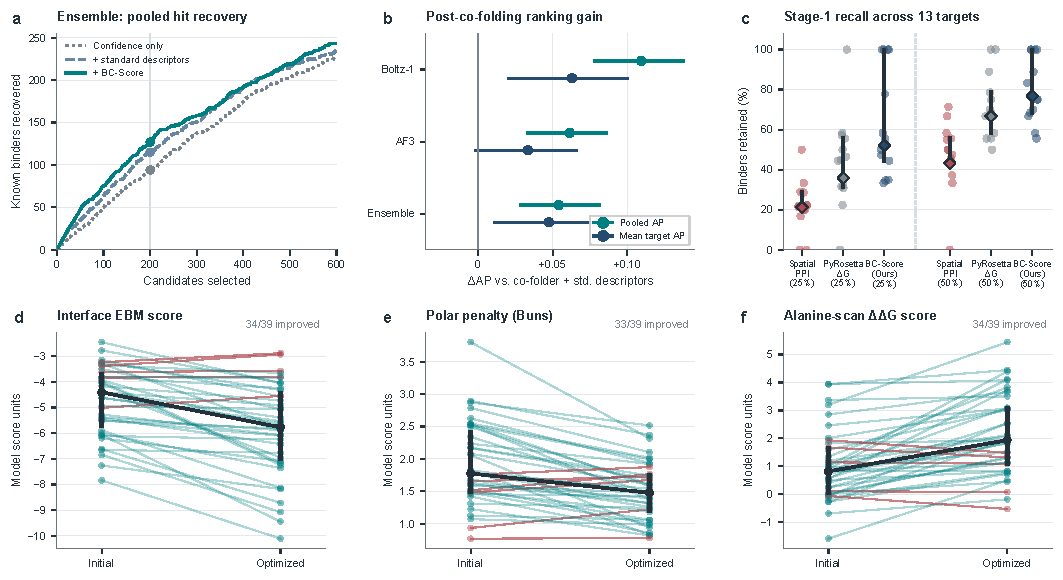
\includegraphics[width=\textwidth]{figures/ext_fig1_supporting_panels.pdf}
\caption{\textbf{Supporting hybrid ranking, Stage-1 cascade recall, and internal optimization analyses.}
\textbf{a}, Pooled retrospective hit recovery across selection budgets for the \texttt{Boltz-1} and \texttt{AlphaFold3} ensemble ($n = 3,532$ complexes, $391$ binders; grey dotted line marks random expectation), comparing confidence alone (grey dashed curve), standard Rosetta descriptors (blue curve), and \texttt{BC-Score} hybrid reranking (solid teal curve). At a budget of $200$ candidates, $94$, $115$, and $127$ binders are recovered, respectively.
\textbf{b}, Point estimates (filled circles) and horizontal error bars showing $95\%$ target-stratified paired bootstrap confidence intervals ($B = 10,000$ resamples across $n = 3,532$ complexes) for $\Delta\text{AP}$ (Pooled AP in teal, 13-target Mean AP in navy; two-sided paired bootstrap $P < 0.001$) when augmenting \texttt{Boltz-1}, \texttt{AlphaFold3}, or their ensemble with \texttt{BC-Score} instead of standard Overath Rosetta physicochemical descriptors.
\textbf{c}, Per-target Stage-1 binder retention distributions across all $13$ targets ($n = 391$ total binders) at retention budgets $\rho = 25\%$ ($4.0\times$ GPU speedup) and $\rho = 50\%$ ($2.0\times$ speedup), showing individual target recall values (jittered circles), interquartile ranges (vertical black lines), and pooled binder recall (filled diamonds) for \texttt{SpatialPPI v2} (red), \texttt{PyRosetta} $\Delta G_{\text{sep}}$ (grey), and \texttt{BC-Score} (navy).
\textbf{d--f}, Paired changes under partition-function free-energy co-design in interface score (\textbf{d}, $34/39$ improved, two-sided Wilcoxon signed-rank $P = 2.1\times 10^{-8}$), buried unsatisfied polar penalty (\textbf{e}, $33/39$ improved, $P = 8.9\times 10^{-8}$), and alanine-scan specificity $\Delta\Delta G$ (\textbf{f}, $34/39$ improved, $P = 2.1\times 10^{-8}$) across $n = 39$ initially failed designs ($3$ per target). Filled teal circles denote improvement, filled red circles denote worsening, and black circles with vertical error bars show medians and interquartile ranges. Values reflect computational objective optimization on fixed backbones prior to experimental retesting.}
\label{fig:focused_support}
\end{figure*}
\clearpage

\begin{figure*}[p]
\centering
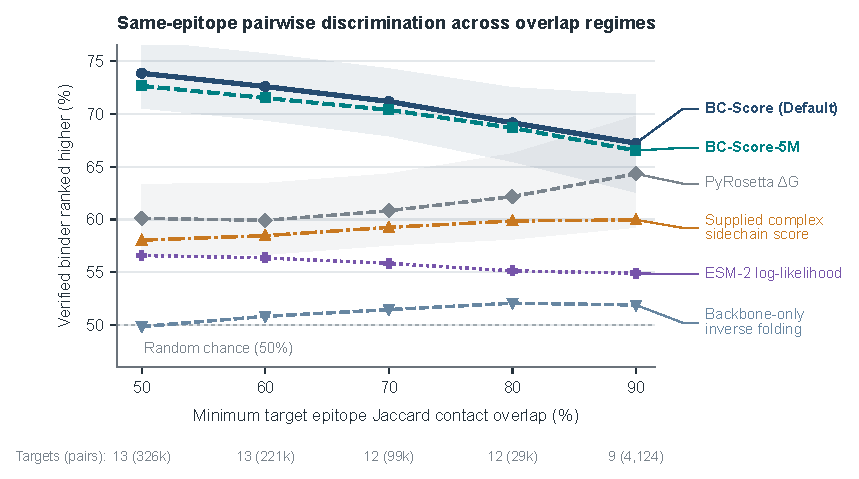
\includegraphics[width=0.92\textwidth]{figures/ext_fig3_same_epitope_pairs.pdf}
\caption{\textbf{Fine-grained pairwise discrimination among same-epitope candidate binders.}
Point estimates and error bars (shaded bands and vertical bars) showing $95\%$ cluster-bootstrap confidence intervals ($1,000$ resamples at the unique candidate binder level across $n = 3,532$ complexes) for pairwise ranking accuracy across all same-target binder and non-binder pairs sharing an increasingly identical receptor contact footprint ($\text{C}_\alpha < 8.5\,\text{\AA}$), from Jaccard contact overlap $\ge 0.50$ ($n = 326,474$ pairs) to $\ge 0.90$ ($n = 4,124$ pairs). Curves compare default \texttt{BC-Score} (solid teal curve with filled circles) and \texttt{BC-Score-5M} (dashed navy curve with open squares) against \texttt{PyRosetta} $\Delta G_{\text{sep}}$ (orange curve), supplied-sidechain scoring (red curve), \texttt{ESM-2} sequence log-likelihood (purple curve), and backbone-only inverse folding (grey curve; horizontal dashed line indicates $50\%$ random chance; two-sided cluster-bootstrap $P < 0.001$ for \texttt{BC-Score} versus all baselines at overlap $\ge 0.50$).}
\label{fig:codesign}
\end{figure*}
\clearpage

\begin{figure*}[p]
\centering
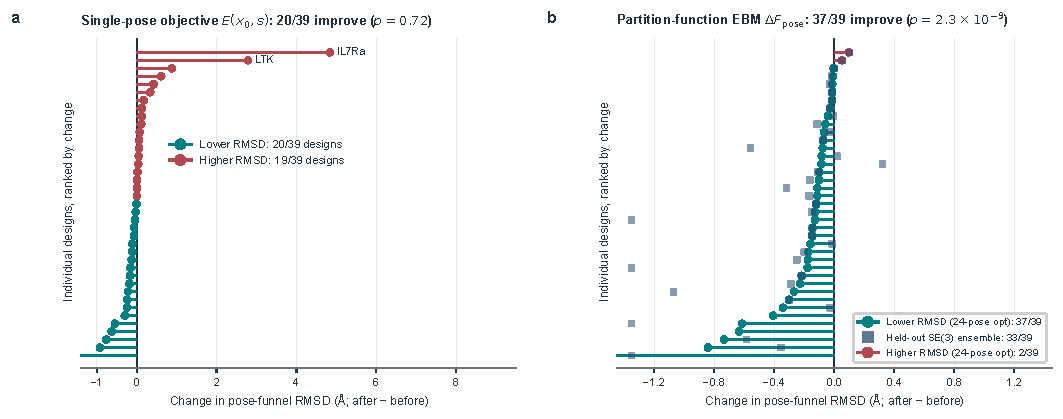
\includegraphics[width=.94\textwidth]{figures/ext_fig2_pose_funnel_codesign.pdf}
\caption{\textbf{Partition-function free-energy co-design resolves the single-pose funnel degradation mode across 39 failed designs.}
\textbf{a}, Paired change in pose-funnel RMSD (after minus before optimization) across all $n = 39$ initially failed Overath designs ($3$ per target) under single-pose coordinate descent ($E(\mathbf{x}_0, \mathbf{s})$), where $20$ designs sharpen the pose funnel (filled teal bars, $\Delta\text{RMSD} < 0$) and $19$ worsen (filled red bars, $\Delta\text{RMSD} > 0$; median $\Delta\text{RMSD} = -0.01\,\text{\AA}$, two-sided Wilcoxon signed-rank $P = 0.72$) due to unpenalized competing decoy basins.
\textbf{b}, Paired change in pose-funnel RMSD across the same $n = 39$ designs under statistical-mechanics partition-function free-energy co-design ($\Delta F_{\text{pose}}(\mathbf{x}_0, \mathbf{s}) = E_\theta(\mathbf{x}_0, \mathbf{s}) - F_{\text{decoy}}(\mathbf{s})$), which sharpens the 24-pose funnel on $\mathbf{37}$ of $\mathbf{39}$ designs (filled teal bars; mean $0.95\,\text{\AA} \to 0.74\,\text{\AA}$, two-sided Wilcoxon signed-rank $P = 2.3\times 10^{-9}$) and generalizes to an independent held-out 24-pose $\text{SE}(3)$ verification ensemble on $\mathbf{33}$ of $\mathbf{39}$ designs (mean $2.22\,\text{\AA} \to 1.06\,\text{\AA}$, $P = 1.3\times 10^{-4}$).}
\label{fig:pose_diagnostic}
\end{figure*}
\clearpage

\begin{table*}[p]
\centering
\caption{\textbf{Held-Out Crystal Sidechain Reconstruction Accuracy ($n = 60$ Validation Monomers, $12,248$ Residues; $n = 50$ Crystal Complexes).} Our 2-Point $\text{SE}(3)$ GNN reconstructs sidechain centroid ($\hat{\mathbf{s}}_i^{\text{recon}}$) and distal functional tip ($\hat{\mathbf{t}}_i^{\text{recon}}$) coordinates strictly from backbone atoms ($\text{N}, \text{C}_\alpha, \text{C}, \text{O}, \text{C}_\beta$) and amino acid identity, outperforming a canonical rigid-backbone local-frame template across all residue classes and at crystal complex interfaces ($<8.5\,\text{\AA}$ $\text{C}_\alpha$ distance). Values report Mean Absolute Error (MAE, in $\text{\AA}$) and the percentage of residues reconstructed within $1.0\,\text{\AA}$ of native crystal coordinates ($P < 10^{-15}$ by two-sided paired Wilcoxon signed-rank test across $n = 12,248$ residues).}
\label{tab:reconstruction}
\footnotesize
\setlength{\tabcolsep}{4.0pt}
\renewcommand{\arraystretch}{1.15}
\resizebox{0.96\textwidth}{!}{%
\begin{tabular}{@{}lcccccc@{}}
\toprule
& \multicolumn{3}{c}{\textbf{Canonical Rigid-Backbone Template}} & \multicolumn{3}{c}{\textbf{Pretrained 2-Point $\text{SE}(3)$ GNN (Ours)}} \\
\cmidrule(lr){2-4} \cmidrule(l){5-7}
\textbf{Residue Subset} & \textbf{Centroid MAE} & \textbf{Tip MAE} & \textbf{Within $1.0\,\text{\AA}$} & \textbf{Centroid MAE} & \textbf{Tip MAE} & \textbf{Within $1.0\,\text{\AA}$} \\
\midrule
All Non-Gly and Non-Ala Monomer Residues ($12,248$) & $0.89\,\text{\AA}$ & $1.59\,\text{\AA}$ & $65.6\%$ & $\mathbf{0.48\,\textbf{\AA}}$ & $\mathbf{0.86\,\textbf{\AA}}$ & $\mathbf{86.0\%}$ \\
Charged Surface and Interface ($\text{Arg, Lys, Asp, Glu}$) & $1.08\,\text{\AA}$ & $2.10\,\text{\AA}$ & $51.4\%$ & $\mathbf{0.68\,\textbf{\AA}}$ & $\mathbf{1.35\,\textbf{\AA}}$ & $\mathbf{76.1\%}$ \\
Polar H-Bonding ($\text{Ser, Thr, Asn, Gln, His}$) & $0.76\,\text{\AA}$ & $1.41\,\text{\AA}$ & $72.6\%$ & $\mathbf{0.43\,\textbf{\AA}}$ & $\mathbf{0.93\,\textbf{\AA}}$ & $\mathbf{92.1\%}$ \\
Bulky Aromatics ($\text{Phe, Trp, Tyr}$) & $2.13\,\text{\AA}$ & $3.81\,\text{\AA}$ & $16.9\%$ & $\mathbf{0.58\,\textbf{\AA}}$ & $\mathbf{0.90\,\textbf{\AA}}$ & $\mathbf{80.6\%}$ \\
Crystal Complex Interface Residues ($<8.5\,\text{\AA}$ $\text{C}_\alpha$) & $1.05\,\text{\AA}$ & --- & $57.4\%$ & $\mathbf{0.57\,\textbf{\AA}}$ & --- & $\mathbf{81.3\%}$ \\
\bottomrule
\end{tabular}%
}
\end{table*}

\begin{table*}[p]
\centering
\caption{\textbf{Complete 13-Fold Leave-One-Target-Out (LOTO) Benchmark and Sensitivity Analysis Across $n = 3,532$ De Novo Binders.} Standalone input-PDB evaluators operate strictly on input design PDB structures without co-folding ($0.043\,\text{s}$ per complex on an NVIDIA A100 GPU for \texttt{BC-Score} versus $35\text{--}180\,\text{s}$ on the same A100 GPU for co-folding). Columns report Pooled Global AP ($n = 3,532$), unweighted 13-target Mean Target AP, 11-target Multi-Hit Mean AP ($n = 3,477$), and Pooled AP excluding \texttt{FGFR2} ($n = 1,409$). Paired differences ($\Delta\text{Global AP}$), $95\%$ confidence intervals, two-sided paired bootstrap $P$ values ($B = 10,000$ target-stratified resamples), and Benjamini--Hochberg FDR $q$-values are reported relative to the reference baseline indicated in each block.}
\label{tab:ext_benchmark}
\footnotesize
\setlength{\tabcolsep}{2.0pt}
\renewcommand{\arraystretch}{1.15}
\resizebox{\textwidth}{!}{%
\begin{tabular}{@{}llccccc@{}}
\toprule
\textbf{Method or Variant} & \begin{tabular}[c]{@{}l@{}}\textbf{Fitted}\\\textbf{Weights}\end{tabular} & \begin{tabular}[c]{@{}c@{}}\textbf{Pooled}\\\textbf{Global AP}\end{tabular} & \begin{tabular}[c]{@{}c@{}}\textbf{Mean Target}\\\textbf{AP (All 13)}\end{tabular} & \begin{tabular}[c]{@{}c@{}}\textbf{Multi-Hit}\\\textbf{AP (11)}\end{tabular} & \begin{tabular}[c]{@{}c@{}}\textbf{Pooled AP}\\\textbf{(Excl.\ FGFR2)}\end{tabular} & \begin{tabular}[c]{@{}c@{}}\textbf{Paired $\Delta\text{Global AP}$}\\\textbf{[95\% CI] ($P$ value; BH $q$)}\end{tabular} \\
\midrule
\multicolumn{7}{@{}l}{\textit{\textbf{Standalone Input-PDB Evaluators (Zero Co-Folding; versus PyRosetta Reference)}}} \\
\hspace{0.4em}\texttt{SpatialPPI v2} (3D GNN) \cite{spatialppi2} & Pretrained & 0.120 & 0.174 & 0.180 & 0.165 & $-0.015$ [$-0.036, +0.005$] ($P = 0.146$; $q = 0.175$) \\
\hspace{0.4em}\texttt{PyRosetta} Interface $\Delta G_{\text{sep}}$ \cite{chaudhury2010pyrosetta} & 0 & 0.135 & 0.267 & 0.272 & 0.198 & Reference (Input PDB) \\
\hspace{0.4em}\texttt{True-EBM} ($M=1$ Cohort-Free Streaming) & 0 & 0.233 & 0.409 & 0.366 & 0.312 & $+0.098$ [$+0.068, +0.129$] ($P < 0.001$; $q = 0.001$) \\
\hspace{0.4em}\texttt{BC-Score-5M} (5-Module, Equal-Weight) & 0 & 0.366 & 0.527 & 0.483 & 0.479 & $+0.230$ [$+0.200, +0.261$] ($P < 0.001$; $q = 0.001$) \\
\hspace{0.4em}\texttt{BC-Score-5M} (5-Module, Nested LOTO) & 5 (Inner) & 0.364 & 0.537 & 0.480 & 0.478 & $+0.229$ [$+0.198, +0.259$] ($P < 0.001$; $q = 0.001$) \\
\hspace{0.4em}\textbf{\texttt{BC-Score} (Default, Equal-Weight)} & \textbf{0} & \textbf{0.383} & \textbf{0.559} & \textbf{0.502} & \textbf{0.487} & \textbf{$+0.248$ [$+0.217, +0.280$] ($P < 0.001$; $q = 0.001$)} \\
\hspace{0.4em}\textbf{\texttt{BC-Score} (Regularized LOTO)} & \textbf{Shrinkage} & \textbf{0.382} & \textbf{0.560} & \textbf{0.503} & \textbf{0.484} & \textbf{$+0.247$ [$+0.218, +0.279$] ($P < 0.001$; $q = 0.001$)} \\
\midrule
\multicolumn{7}{@{}l}{\textit{\textbf{Standalone GPU Co-Folding Baselines (versus Standalone BC-Score Default Reference)}}} \\
\hspace{0.4em}\texttt{AlphaFold2-Initial-Guess iPAE} \cite{bennett2023improving} & 0 & 0.242 & 0.398 & 0.341 & 0.242 & $-0.140$ [$-0.172, -0.109$] ($P < 0.001$; $q = 0.001$) \\
\hspace{0.4em}\texttt{ColabFold AF2-Multimer ipSAE} \cite{mirdita2022colabfold,dunbrack2025ipsae} & 0 & 0.289 & 0.376 & 0.412 & 0.327 & $-0.093$ [$-0.129, -0.057$] ($P < 0.001$; $q = 0.001$) \\
\hspace{0.4em}\texttt{ColabFold AF2-Multimer actifpTM} \cite{varga2025actifptm} & 0 & 0.295 & 0.380 & 0.425 & 0.357 & $-0.087$ [$-0.128, -0.046$] ($P < 0.001$; $q = 0.001$) \\
\hspace{0.4em}\texttt{Boltz-1 ipSAE} \cite{wohlwend2024boltz1,dunbrack2025ipsae} & 0 & 0.336 & 0.425 & 0.430 & 0.353 & $-0.046$ [$-0.086, -0.004$] ($P = 0.036$; $q = 0.046$) \\
\hspace{0.4em}\texttt{AlphaFold3 ipTM} \cite{abramson2024accurate} & 0 & 0.319 & 0.480 & 0.466 & 0.346 & $-0.063$ [$-0.102, -0.024$] ($P = 0.004$; $q = 0.006$) \\
\hspace{0.4em}\texttt{AlphaFold3 LIS} \cite{kim2024lis} & 0 & 0.350 & 0.506 & 0.496 & 0.362 & $-0.032$ [$-0.077, +0.009$] ($P = 0.126$; $q = 0.162$) \\
\hspace{0.4em}\texttt{AlphaFold3 ipSAE} \cite{abramson2024accurate,dunbrack2025ipsae} & 0 & 0.361 & 0.545 & 0.543 & 0.390 & $-0.022$ [$-0.064, +0.023$] ($P = 0.338$; $q = 0.375$) \\
\midrule
\multicolumn{7}{@{}l}{\textit{\textbf{Post-Co-Fold Hybrid Evaluators (versus Respective Raw Co-Folder Reference)}}} \\
\hspace{0.4em}\texttt{Boltz-1} + Std.\ \texttt{Rosetta} Phys.\ \cite{overath2025predicting} & LOTO & 0.339 & 0.457 & 0.467 & 0.330 & $+0.003$ [$-0.019, +0.025$] ($P = 0.780$; $q = 0.780$) \\
\hspace{0.4em}\textbf{\texttt{Boltz-1} + \texttt{BC-Score} (Ours)} & \textbf{LOTO} & \textbf{0.449} & \textbf{0.520} & \textbf{0.542} & \textbf{0.474} & \textbf{$+0.113$ [$+0.078, +0.145$] ($P < 0.001$; $q = 0.001$)} \\
\hspace{0.4em}\texttt{AlphaFold3} + Std.\ \texttt{Rosetta} Phys.\ \cite{overath2025predicting} & LOTO & 0.407 & 0.577 & 0.581 & 0.439 & $+0.046$ [$+0.019, +0.074$] ($P < 0.001$; $q = 0.001$) \\
\hspace{0.4em}\textbf{\texttt{AlphaFold3} + \texttt{BC-Score} (Ours)} & \textbf{LOTO} & \textbf{0.468} & \textbf{0.611} & \textbf{0.620} & \textbf{0.537} & \textbf{$+0.107$ [$+0.072, +0.138$] ($P < 0.001$; $q = 0.001$)} \\
\hspace{0.4em}\texttt{Boltz-1 + AF3} (Raw Ensemble) & 0 & 0.372 & 0.523 & 0.541 & 0.396 & Reference (Ensemble) \\
\hspace{0.4em}\texttt{Boltz-1 + AF3} + Std.\ \texttt{Rosetta} Phys. & LOTO & 0.454 & 0.530 & 0.549 & 0.450 & $+0.082$ [$+0.051, +0.112$] ($P < 0.001$; $q = 0.001$) \\
\hspace{0.4em}\textbf{\texttt{Boltz-1 + AF3} + \texttt{BC-Score} (Ours)} & \textbf{LOTO} & \textbf{0.508} & \textbf{0.577} & \textbf{0.604} & \textbf{0.550} & \textbf{$+0.136$ [$+0.103, +0.169$] ($P < 0.001$; $q = 0.001$)} \\
\bottomrule
\end{tabular}%
}
\end{table*}
\clearpage

\begin{table*}[p]
\centering
\caption{\textbf{Retrospective Two-Stage Screening Cascade Simulation Across $n = 3,532$ Candidates and $13$ Targets ($391$ Verified Binders).} For each Stage-1 filter and per-target retention fraction $\rho$, candidates are ranked within each target by their out-of-fold Stage-1 score, and only the top $\lceil \rho N_t \rceil$ survivors are passed to Stage-2 \texttt{AlphaFold3} co-folding ($180\,\text{s}$ per complex on an NVIDIA A100 GPU). Columns report Stage-1 pooled binder recall, across-target mean and median recall ($n = 13$ targets), and verified binders recovered in the Top-10 per target (maximum $130$) and Global Top-200 (in parentheses). Per-target recall distributions are shown in Extended Data Fig.~\ref{fig:focused_support}c.}
\label{tab:cascade}
\footnotesize
\setlength{\tabcolsep}{3.0pt}
\renewcommand{\arraystretch}{1.15}
\resizebox{\textwidth}{!}{%
\begin{tabular}{@{}llccccc@{}}
\toprule
\textbf{Stage-1 Filter} & \begin{tabular}[c]{@{}l@{}}\textbf{Co-Fold}\\\textbf{Budget $\rho$ ($n$)}\end{tabular} & \begin{tabular}[c]{@{}c@{}}\textbf{Total Compute}\\\textbf{(GPU Reduction)}\end{tabular} & \begin{tabular}[c]{@{}c@{}}\textbf{Stage-1}\\\textbf{Pooled Recall}\end{tabular} & \begin{tabular}[c]{@{}c@{}}\textbf{Target Recall}\\\textbf{(Mean, Median)}\end{tabular} & \begin{tabular}[c]{@{}c@{}}\textbf{AF3 Alone}\\\textbf{Top-10/T (Top-200)}\end{tabular} & \begin{tabular}[c]{@{}c@{}}\textbf{AF3 + BC-Score}\\\textbf{Top-10/T (Top-200)}\end{tabular} \\
\midrule
\multicolumn{7}{@{}l}{\textit{\textbf{Reference Workflow: Co-Fold 100\% of Candidates (No Pre-Filter)}}} \\
\hspace{0.4em}None (100\% Co-Folded) & 100\% (3,532) & 176.6\,h GPU ($1.0\times$) & 100.0\% & 100.0\%, 100.0\% & 67 (89) & \textbf{74 (123)} \\
\midrule
\multicolumn{7}{@{}l}{\textit{\textbf{Zero Co-Folding Workflows (Stage-1 Filter Alone; 0\% Co-Folded)}}} \\
\hspace{0.4em}\texttt{SpatialPPI v2} Alone & 0\% (0) & 1.8\,h CPU & --- & --- & 20 (32) & --- \\
\hspace{0.4em}\texttt{PyRosetta} $\Delta G_{\text{sep}}$ Alone & 0\% (0) & 4.4\,h CPU & --- & --- & 33 (25) & --- \\
\hspace{0.4em}\textbf{\texttt{BC-Score} (Default, Equal) Alone} & \textbf{0\% (0)} & \textbf{0.042\,h GPU ($4,176\times$)} & --- & --- & \textbf{56 (111)} & --- \\
\hspace{0.4em}\textbf{\texttt{BC-Score} (Reg.\ LOTO) Alone} & \textbf{0\% (0)} & \textbf{0.042\,h GPU ($4,176\times$)} & --- & --- & \textbf{58 (110)} & --- \\
\midrule
\multicolumn{7}{@{}l}{\textit{\textbf{Two-Stage Screening Cascade at $\rho = 25\%$ Co-Folding Budget ($4.0\times$ Fewer GPU Calls)}}} \\
\hspace{0.4em}\texttt{SpatialPPI v2} $\to$ Co-Fold & 25\% (888) & 44.4\,h GPU ($4.0\times$) & 21.2\% & 21.9\%, 21.8\% & 35 (52) & 29 (55) \\
\hspace{0.4em}\texttt{PyRosetta} $\Delta G_{\text{sep}}$ $\to$ Co-Fold & 25\% (888) & 44.4\,h GPU ($4.0\times$) & 35.8\% & 44.1\%, 45.0\% & 55 (92) & 59 (88) \\
\hspace{0.4em}\textbf{\texttt{BC-Score} (Default) $\to$ Co-Fold} & \textbf{25\% (888)} & \textbf{44.4\,h GPU ($4.0\times$)} & \textbf{52.2\%} & \textbf{64.3\%, 55.4\%} & \textbf{66 (113)} & \textbf{69 (119)} \\
\hspace{0.4em}\textbf{\texttt{BC-Score} (Reg.\ LOTO) $\to$ Co-Fold} & \textbf{25\% (888)} & \textbf{44.4\,h GPU ($4.0\times$)} & \textbf{52.7\%} & \textbf{64.6\%, 56.0\%} & \textbf{67 (116)} & \textbf{69 (119)} \\
\midrule
\multicolumn{7}{@{}l}{\textit{\textbf{Two-Stage Screening Cascade at $\rho = 40\%$ and $\rho = 50\%$ Co-Folding Budgets ($2.5\times$ and $2.0\times$ Fewer GPU Calls)}}} \\
\hspace{0.4em}\texttt{SpatialPPI v2} $\to$ Co-Fold & 50\% (1,770) & 88.5\,h GPU ($2.0\times$) & 43.2\% & 47.3\%, 50.0\% & 54 (85) & 54 (79) \\
\hspace{0.4em}\texttt{PyRosetta} $\Delta G_{\text{sep}}$ $\to$ Co-Fold & 50\% (1,770) & 88.5\,h GPU ($2.0\times$) & 66.8\% & 71.8\%, 68.4\% & 64 (102) & 70 (111) \\
\hspace{0.4em}\textbf{\texttt{BC-Score} (Default) $\to$ Co-Fold} & \textbf{40\% (1,419)} & \textbf{71.0\,h GPU ($2.5\times$)} & \textbf{65.5\%} & \textbf{73.3\%, 71.0\%} & \textbf{71 (107)} & \textbf{71 (120)} \\
\hspace{0.4em}\textbf{\texttt{BC-Score} (Default) $\to$ Co-Fold} & \textbf{50\% (1,770)} & \textbf{88.5\,h GPU ($2.0\times$)} & \textbf{76.7\%} & \textbf{80.1\%, 75.0\%} & \textbf{75 (107)} & \textbf{72 (122)} \\
\hspace{0.4em}\textbf{\texttt{BC-Score} (Reg.\ LOTO) $\to$ Co-Fold} & \textbf{50\% (1,770)} & \textbf{88.5\,h GPU ($2.0\times$)} & \textbf{76.7\%} & \textbf{80.0\%, 75.0\%} & \textbf{75 (107)} & \textbf{72 (122)} \\
\bottomrule
\end{tabular}%
}
\end{table*}
\clearpage

\begin{table*}[p]
\centering
\caption{\textbf{Held-Out External Validation on Two Public Experimental Campaigns.} All \texttt{BC-Score} feature definitions, signs, checkpoints, and Overath-fitted normalization parameters were frozen prior to evaluation and applied without modification. On \texttt{Nipah-G} (\texttt{nipah-binder-competition-results}; $n = 881$ \texttt{Boltz-2}-predicted complexes \cite{passaro2025boltz2}, $100$ binders), Pooled AP is shown with $95\%$ bootstrap confidence intervals ($B = 10,000$ resamples) in brackets, alongside AUROC and top-$K$ hit recovery at $K=25$ and $K=50$. On \texttt{Scorpion} (\texttt{Anthropic/scorpion-toxin-binder-design}; $n = 243$ raw upstream pre-co-fold design PDB structures across $5$ targets; \texttt{ESMFold2} denotes the CZ Biohub \texttt{ESMFold2} complex predictor \cite{candido2026esmfold2}), point estimates are reported across all $21$ Adaptyv Bio binding hits with sensitivity point estimates on the $12$ Twist-confirmed publication hits shown in brackets, and top-$K$ recovery is reported at $K=20$ and $K=50$.}
\label{tab:external}
\footnotesize
\setlength{\tabcolsep}{2.8pt}
\renewcommand{\arraystretch}{1.15}
\resizebox{\textwidth}{!}{%
\begin{tabular}{@{}llccccc@{}}
\toprule
\textbf{Campaign and Method} & \begin{tabular}[c]{@{}l@{}}\textbf{Input and}\\\textbf{Category}\end{tabular} & \begin{tabular}[c]{@{}c@{}}\textbf{Pooled AP}\\\textbf{[Nipah 95\% CI /}\\\textbf{Scorpion 12-Hit Pub]}\end{tabular} & \begin{tabular}[c]{@{}c@{}}\textbf{Mean Target AP}\\\textbf{[Scorpion 12-Hit}\\\textbf{Pub]}\end{tabular} & \textbf{AUROC} & \begin{tabular}[c]{@{}c@{}}\textbf{Top-25 or}\\\textbf{Top-20 Hits}\end{tabular} & \begin{tabular}[c]{@{}c@{}}\textbf{Top-50}\\\textbf{Hits}\end{tabular} \\
\midrule
\multicolumn{7}{@{}l}{\textit{\textbf{External Campaign 1: Adaptyv Bio Nipah-G ($n = 881$ Boltz-2 Complexes, $100$ Binders [11.35\%], 1 Target; Brackets = 95\% Bootstrap CI)}}} \\
\hspace{0.4em}\texttt{ProteinMPNN} Sequence Score \cite{dauparas2022robust} & Sequence Log-Prob & 0.100 [0.083, 0.124] & 0.100 & 0.479 & 1 / 25 (4\%) & 2 / 50 (4\%) \\
\hspace{0.4em}\texttt{Boltz-2 pDockQ2} \cite{zhu2023pdockq2} & GPU Co-Folder Metric & 0.114 [0.093, 0.134] & 0.114 & 0.500 & 4 / 25 (16\%) & 4 / 50 (8\%) \\
\hspace{0.4em}\texttt{ESMFold} Monomer pLDDT \cite{lin2023evolutionary} & Fast Monomer Fold & 0.124 [0.097, 0.170] & 0.124 & 0.548 & 2 / 25 (8\%) & 3 / 50 (6\%) \\
\hspace{0.4em}\texttt{Boltz-2 LIS} \cite{kim2024lis} & GPU Co-Folder Metric & 0.131 [0.105, 0.167] & 0.131 & 0.583 & 0 / 25 (0\%) & 0 / 50 (0\%) \\
\hspace{0.4em}\texttt{Boltz-2 ipTM} \cite{passaro2025boltz2} & GPU Co-Folder Metric & 0.136 [0.108, 0.178] & 0.136 & 0.587 & 2 / 25 (8\%) & 4 / 50 (8\%) \\
\hspace{0.4em}\texttt{Boltz-2 Complex pLDDT} \cite{passaro2025boltz2} & GPU Co-Folder Metric & 0.146 [0.115, 0.202] & 0.146 & 0.594 & 5 / 25 (20\%) & 7 / 50 (14\%) \\
\hspace{0.4em}\textbf{\texttt{BC-Score} (Default, Equal) [Locked]} & \textbf{Boltz-2 Struct ($0.041\,\text{s}$)} & \textbf{0.155 [0.116, 0.213]} & \textbf{0.155} & \textbf{0.567} & \textbf{3 / 25 (12\%)} & \textbf{10 / 50 (20\%)} \\
\hspace{0.4em}\textbf{\texttt{BC-Score} (Reg.\ LOTO) [Locked]} & \textbf{Boltz-2 Struct ($0.041\,\text{s}$)} & \textbf{0.156 [0.118, 0.217]} & \textbf{0.156} & \textbf{0.563} & \textbf{4 / 25 (16\%)} & \textbf{11 / 50 (22\%)} \\
\hspace{0.4em}\texttt{True-EBM} ($M=1$ Streaming) & Boltz-2 Struct ($0.041\,\text{s}$) & 0.182 [0.135, 0.244] & 0.182 & 0.594 & 5 / 25 (20\%) & 11 / 50 (22\%) \\
\hspace{0.4em}\texttt{Boltz-2 ipSAE} \cite{passaro2025boltz2,dunbrack2025ipsae} & GPU Co-Folder Metric & 0.193 [0.142, 0.262] & 0.193 & 0.622 & 7 / 25 (28\%) & 9 / 50 (18\%) \\
\hspace{0.4em}\texttt{Boltz-2} $\min\text{ipSAE}$ \cite{dunbrack2025ipsae} & GPU Co-Folder Metric & \textbf{0.229 [0.164, 0.299]} & \textbf{0.229} & \textbf{0.645} & \textbf{9 / 25 (36\%)} & 10 / 50 (20\%) \\
\hspace{0.4em}\textbf{Hybrid: \texttt{Boltz-2 ipSAE + BC-Score}} & \textbf{Post-Co-Fold Rerank} & \textbf{0.229 [0.162, 0.311]} & \textbf{0.229} & \textbf{0.618} & \textbf{8 / 25 (32\%)} & \textbf{16 / 50 (32\%)} \\
\midrule
\multicolumn{7}{@{}l}{\textit{\textbf{External Campaign 2: Anthropic and Adaptyv Scorpion Neurotoxins ($n = 243$ Raw PDBs, 5 Targets; 21 Adaptyv [12 Pub] Hits)}}} \\
\hspace{0.4em}\texttt{Protenix-V2 ipSAE} (AF3 Reprod.) \cite{bytedance2025protenix} & GPU Co-Folder & 0.226 [0.174] & 0.262 [0.224] & 0.748 & 5 / 20 [3/20] & 11 / 50 [7/50] \\
\hspace{0.4em}\texttt{Protenix-V2 scDockQ} \cite{bytedance2025protenix,basu2016dockq} & GPU Co-Folder & 0.222 [0.145] & 0.305 [0.211] & 0.805 & 2 / 20 [1/20] & 14 / 50 [9/50] \\
\hspace{0.4em}\texttt{ESMFold2 scDockQ} \cite{candido2026esmfold2,basu2016dockq} & Fast Complex Fold & 0.231 [0.153] & 0.290 [0.219] & 0.819 & 5 / 20 [3/20] & 13 / 50 [7/50] \\
\hspace{0.4em}Campaign Multi-Oracle Composite & Multi-Oracle Pipeline & 0.264 [0.186] & 0.329 [0.296] & \textbf{0.824} & 5 / 20 [2/20] & 14 / 50 [10/50] \\
\hspace{0.4em}\texttt{ESMFold2 ipSAE} \cite{candido2026esmfold2,dunbrack2025ipsae} & Fast Complex Fold & 0.336 [0.289] & 0.377 [0.386] & 0.823 & 8 / 20 [6/20] & 16 / 50 [11/50] \\
\hspace{0.4em}\textbf{\texttt{BC-Score} (Default, Equal) [Locked]} & \textbf{Raw PDB ($0.038\,\text{s}$)} & \textbf{0.141 [0.104]} & \textbf{0.319 [0.448]} & \textbf{0.618} & \textbf{3 / 20 [2/20]} & \textbf{7 / 50 [4/50]} \\
\hspace{0.4em}\texttt{BC-Score-5M} (5-Module, Equal) [Locked] & Raw PDB ($0.038\,\text{s}$) & 0.170 [0.165] & 0.408 [0.599] & 0.609 & 3 / 20 [2/20] & 7 / 50 [5/50] \\
\hspace{0.4em}\texttt{True-EBM} ($M=1$ Streaming) & Raw PDB ($0.038\,\text{s}$) & 0.152 [0.123] & 0.306 [0.424] & 0.651 & 3 / 20 [3/20] & 8 / 50 [5/50] \\
\hspace{0.4em}\textbf{Hybrid: \texttt{Protenix-V2 + BC-Score}} & \textbf{Post-Co-Fold Rerank} & \textbf{0.288 [0.275]} & \textbf{0.367 [0.415]} & \textbf{0.706} & \textbf{8 / 20 [6/20]} & \textbf{11 / 50 [8/50]} \\
\hspace{0.4em}\textbf{Hybrid: \texttt{ESMFold2 + BC-Score}} & \textbf{Post-Co-Fold Rerank} & \textbf{0.376 [0.365]} & \textbf{0.463 [0.527]} & \textbf{0.785} & \textbf{10 / 20 [8/20]} & \textbf{13 / 50 [9/50]} \\
\bottomrule
\end{tabular}%
}
\end{table*}
\clearpage

\end{document}
